\documentclass[conference,a4paper]{IEEEtran}
\usepackage[T1]{fontenc}
\usepackage[utf8]{inputenc}
\usepackage{amsmath,amssymb,graphicx,booktabs,array,microtype}
\usepackage[authoryear,round]{natbib}
\usepackage{xcolor}
\usepackage{xurl}
\usepackage[colorlinks=true,urlcolor=blue!55!black,citecolor=blue!55!black,linkcolor=blue!55!black]{hyperref}
\setlength{\emergencystretch}{2em}
\newcommand{\fig}[3]{\begin{figure}[t]\centering\includegraphics[width=\columnwidth]{images/#1.pdf}\caption{#2}\label{#3}\end{figure}}
\newcommand{\widefig}[3]{\begin{figure}[tbp]\centering\includegraphics[width=\columnwidth]{images/#1.pdf}\caption{#2}\label{#3}\end{figure}}
\title{Predicting Next-Day Forest Fire Detections in Nepal Using Machine Learning}
\author{\IEEEauthorblockN{Krijal Shrestha}\IEEEauthorblockA{Coventry ID: 11495103\\STW7072CEM Machine Learning\\Softwarica College of IT and E-commerce, Coventry University}}

\begin{document}
\maketitle
\begin{abstract}
Forest-fire prediction in Nepal requires models that can identify uncommon fire days from incomplete satellite records and environmental data. This study uses ICIMOD's Active Fire Incidents in Nepal dataset, containing MODIS detections from February 2012 to June 2016. These records are combined with ERA5 daily weather for 2012--2016 accessed through Open-Meteo, Nepal's 2011 forest-cover map, SRTM elevation acquired in 2000 and a national boundary. Cleaning and geographic integration produce a daily dataset for 238 forest-containing grid cells. Logistic Regression provides a linear benchmark, Linear Support Vector Machine tests margin-based classification, Random Forest captures feature interactions, and Gradient Boosting tests sequential tree learning. Training uses 2012--2014, validation uses 2015 and testing uses January--June 2016. Class weighting addresses imbalance in the main comparison; separate experiments test whether PCA or SMOTE improves Logistic Regression. Linear SVM leads validation ranking, while the tree ensembles perform better on several later test measures. PCA and SMOTE do not improve validation ranking over the weighted comparator. The outputs are fitted classifiers, daily detection scores, a historical ranking map and a reproducible comparison of model performance. The findings support further development while showing why uncertain absence labels and variation across years limit operational use.

\end{abstract}
\begin{IEEEkeywords}
Nepal, ICIMOD, forest fire, class imbalance, support vector machine, SMOTE, principal component analysis
\end{IEEEkeywords}

\section{Introduction}
Forest fires damage forest ecosystems, threaten nearby communities and affect the carbon and biodiversity held in Nepal's forests \citep{dahal}. Understanding where and when fires may occur can support monitoring and preparedness. Weather affects environmental conditions, while forest cover and terrain help distinguish locations. Satellite observations provide records of detected fires, but they are affected by clouds, overpass times and archive completeness. A prediction model must therefore learn from useful environmental information while accounting for uncertainty in its outcome labels.

This study uses Active Fire Incidents in Nepal, distributed through ICIMOD's Regional Database System \citep{icimodfire}. ICIMOD is an intergovernmental institution headquartered in Kathmandu \citep{icimodabout}; MODIS supplies the underlying satellite observations. The regional dataset is relevant to Nepal, but it does not independently confirm every fire or establish fire-free conditions whenever a record is absent.

The study compares four classifiers using the same prepared dataset and chronological partitions. It retains Logistic Regression, Random Forest and Gradient Boosting from the proposal and adds Linear SVM to test a different learning objective. The comparison asks which models discriminate recorded fire days most effectively and whether extra preprocessing improves that performance. Actual source checks, model settings and prediction errors provide the basis for the discussion.

\subsection{Aim}
The aim is to develop and compare machine-learning models for next-day recorded forest-fire detection in Nepal using ICIMOD incidents, preceding weather and geographic data.

\subsection{Prediction Task and Study Contribution}
For target day $t$, the model uses weather ending on $t-1$ to estimate whether a forest-containing grid cell will have at least one retained detection. A prediction for 15 April therefore uses weather through 14 April. A threshold chosen on validation data converts its score into a binary decision. A negative label means that no retained detection was recorded for that cell-day.

The contribution is a common daily dataset, four applied classifiers and controlled tests of preprocessing choices. The study distinguishes the model chosen on validation data from the strongest model observed later. This is important because 2015 contains unusually few positive records. PCA and SMOTE are supplementary experiments whose usefulness is measured rather than assumed.

\section{Literature Review}
\subsection{Forest-Fire Mapping in Nepal}
\citet{dhakal} compare fuzzy analytical hierarchy process, Random Forest and boosted regression trees in Nepal's Chure Tarai Madhesh Landscape. Their study links fire mapping to environmental conditions and compares expert judgement with learned relationships. It motivates the use of several methods rather than assuming that one algorithm will be suitable everywhere. For the present task, the main limitation of transferring their findings is the difference between spatial susceptibility and next-day recorded detection. A location can be susceptible over several years without a fire being observed on a particular day. The research gap addressed here is therefore a temporal evaluation question: how do different classifiers behave when predictors precede the target and evaluation moves to a later year? The proposed response is a common grid-day dataset and chronological comparison. This extends the application rather than reproducing their expert-weighted mapping method.

\citet{dahal} examine Nepal's forest-fire patterns and susceptibility in relation to carbon stocks and biodiversity. Their work gives the prediction problem an ecological context: the consequences of fire extend beyond the number of recorded locations. Its strength is the link between spatial fire information and resources potentially exposed to damage. However, those outcomes are broader than the binary daily label available in this project. The present study has neither burned-area measurements nor carbon-loss or species-impact labels. Its response is to keep the outcome narrow and measurable, while investigating whether preceding weather helps distinguish daily recorded events. The limitation is explicit: better classification of detections would not by itself quantify ecological damage or establish a benefit for biodiversity conservation.

\subsection{Regional Model Comparisons}
\citet{sarkar} compare boosted regression trees, Random Forest, SVM, classification and regression trees, multivariate adaptive regression splines and an ensemble for Northeast India. They use VIIRS fire locations from 2018--2019, giving the study a different sensor, period and regional setting from the MODIS-based ICIMOD export. The comparative design supports examining several model families. Its results do not establish daily predictive performance in Nepal. The short source period also motivates caution about temporal generalisation. The response here is to train on Nepal-specific observations, use weather from preceding days and examine later-year and geographic diagnostics. The implemented SVM is linear, so this is not a replication of all the configurations in the regional study. Reported susceptibility scores from that paper are not treated as directly comparable benchmarks for this daily task.

\subsection{Imbalance, Representation and Evaluation}
The literature also informs how the comparison should be assessed. \citet{saito} explain why precision--recall analysis is useful when one class is rare. ROC-AUC describes how positive and negative cases are ranked, but a large negative class can leave the practical burden of false alarms unclear. This study therefore reports precision, recall, F1 and average precision alongside ordinary and balanced accuracy. Average precision summarises ranking across thresholds; F1 describes a particular decision threshold. A model may perform differently on these measures, so they cannot be combined into one interchangeable notion of accuracy.

SMOTE addresses imbalance by interpolating between minority examples \citep{chawla}. It can give the learner more minority-class representation, but it adds synthetic points rather than new observed fires. The imbalanced-learn framework supports placing this operation inside a training pipeline \citep{lemaitre}. This matters because resampling before dividing the data could allow evaluation information into the fitted model. PCA addresses a different problem: correlated predictors can be represented by fewer orthogonal components \citep{jolliffe}. It preserves variation in the predictors, not necessarily information most useful for a rare target. Both techniques therefore require an empirical comparison against an appropriate baseline.

Dependence between nearby dates and places is another concern. \citet{roberts} show why evaluation of structured ecological data needs to respect the intended prediction setting. Here, the main split tests later dates at known cells, while a geographic diagnostic asks a different transfer question. Neither is replaced by randomly mixing all grid-days. The research gap is the relative performance of these classifiers and preprocessing strategies on the supplied ICIMOD daily task under temporal and geographic evaluation.
\section{Study Data and Problem Definition}
\subsection{ICIMOD Active Fire Incidents in Nepal}
The primary dataset contains 13,781 rows and 25 columns, dated 1 February 2012--19 June 2016. Coordinates, acquisition date and time, satellite identifier and confidence support cleaning and target construction. Brightness, fire radiative power, land-cover descriptors and administrative attributes are also present. The ICIMOD catalogue identifies the MODIS origin, Nepal coverage and Creative Commons Attribution licence \citep{icimodfire}. The original CSV is preserved and identified by a checksum.

The records range from 26.426 to 30.10937 degrees north and 80.10448 to 88.16501 degrees east. One fire can generate several satellite detections, so records are aggregated by cell and day. Annual source counts are 3,149 in 2012, 1,999 in 2013, 2,386 in 2014, 489 in 2015 and 5,758 in 2016. The endpoint years are partial. The low 2015 count cannot be attributed confidently to fewer fires, observation differences or archive gaps; its effect on validation is considered explicitly.

\subsection{Environmental Data and Their Roles}
Open-Meteo's Historical Weather API supplies ERA5 data for 1 January 2012--31 December 2016 \citep{openmeteo,hersbach}. The seven daily variables are mean and maximum 2-m temperature, precipitation sum, mean and minimum relative humidity, and mean and maximum 10-m wind speed. Units are degrees Celsius, millimetres, percentage humidity and metres per second. Requests use Asia/Kathmandu aggregation, nearest-cell selection and disabled elevation adjustment. These settings provide consistent daily inputs for recent-weather features.

ERA5 at nominal 0.25-degree spacing replaces the proposal's ERA5-Land route. The products are not mixed: humidity and wind summaries are supplied by the service rather than derived here from hourly dewpoint and vector components. This change retains the intended environmental predictors but uses a different source resolution and processing route.

The Forest Research and Training Centre's 2011 land-cover layer, distributed through ICIMOD, defines forest as class 4 \citep{frtc}. The same mask determines eligible cells and retained detections. Later collected maps are excluded to keep one pre-study definition; no 2012 layer was supplied. Because the collection was produced retrospectively, this choice does not establish that the map was available operationally in 2011.

The approximately 30-m SRTM GL1 raster, downloaded through OpenTopography, supplies elevation and derived slope and aspect summaries. Its acquisition dates to February 2000 \citep{srtm}. These features describe terrain context, not annual change or weather at 30-m resolution. The geoBoundaries ADM0 polygon restricts the analysis to the supplied Nepal boundary \citep{runfola}. Its metadata identify a 2019 representation. It defines the footprint rather than reconstructing historical boundary changes.

\subsection{Analytical Grid and Target}
All 238 requested forest-containing grid locations have complete weather histories. Each contains 1,827 unique daily dates from 1 January 2012 to 31 December 2016, with all seven variables present and finite. The response metadata also identify 238 distinct returned weather cells. Thus, the location requests do not merely repeat one weather series under different requested coordinates. The source-file hashes and grid identifiers are recorded in a manifest for the full-data run.

Let $g$ identify an eligible cell and $t$ a local calendar day. The target is
\begin{equation}
y_{g,t}=\mathbb{1}\!\left\{\text{at least one retained detection in }(g,t)\right\}.
\end{equation}
A zero means no retained recorded detection, not confirmed absence. The data retain all eligible grid-days, rather than selecting a matched sample of negative records. This preserves the observed class prevalence within the analysis footprint. A cell centre can lie outside the boundary while its cell intersects forest inside Nepal; eligibility is determined by forest pixels within the polygon, not by centre-point nationality.

\widefig{coverage_counts}{Study footprint and source counts. Colours show retained positive grid-days across the analysed forest-grid cells. Counts in the right panel are source rows before cleaning; 2012 and 2016 are partial years.}{fig:coverage}

\section{Data Preparation and Feature Engineering}
\subsection{Cleaning and Integration}
The source audit finds no exact duplicate rows or invalid latitude and longitude values. District, zone and VDC each have one missing entry; the protected-area field has 11,437. These fields are excluded from prediction, so their missing entries are not imputed. Acquisition dates and times pass the implemented validity checks. MODIS-style time is interpreted as UTC and converted to Asia/Kathmandu before daily aggregation; this convention remains an assumption about the supplied export.

Detections are ordered by confidence and deduplicated using coordinates rounded to five decimal places, timestamp and satellite. This removes 224 repeated detection keys while retaining the highest-confidence version. A whole-row duplicate check would not identify these records. The rule removes repeated observations without attempting to reconstruct individual multi-pixel fires. One point is outside the Nepal polygon. Applying forest class 4 removes another 3,298 points, leaving 10,258 forest-detection rows before model-date restrictions and aggregation.

Each weather file is checked for the exact expected dates, repeated dates, grid identity and finite numeric values. Rainfall is nonnegative, mean humidity lies between zero and one hundred, daily maximum temperature and wind are not below their means, and minimum humidity is not above the mean. Prepared predictors have no missing values; imputation is therefore unnecessary. Plausible extreme weather is retained rather than removed using an arbitrary normal-distribution rule.

Points are assigned to the nearest nominal quarter-degree cell and joined with weather by cell identifier and local date. Multiple detections become one positive cell-day. The first and last source dates are excluded because complete observation at those endpoints is not established. The model interval is 2 February 2012--18 June 2016, yielding 380,562 rows with 4,399 positive cell-days and no repeated cell-date keys.

Terrain processing aligns elevation to the land-cover raster by bilinear resampling. Slope uses local metre distances when calculating elevation gradients, with overlapping processing rows to avoid artificial block edges. Elevation, slope, northness and eastness are averaged over forest pixels inside Nepal. Forest fraction divides forest-pixel counts by classified-pixel counts within each clipped cell. These operations put the spatial layers on a common analytical grid without claiming that every pixel shares its cell's average conditions.

\subsection{Predictors and mathematical construction}
Twenty-one predictors are used. Six are previous-day mean and maximum temperature, mean and minimum humidity, and mean and maximum wind speed. Three describe preceding precipitation totals over one, seven and thirty days. Two give preceding seven-day temperature and humidity means. One represents the preceding dry-day run. The remaining nine are latitude, longitude, forest fraction, mean elevation, mean slope, mean aspect northness and eastness, and sine/cosine seasonal terms.

For precipitation $P$, the rolling predictor is
\begin{equation}
R^{(k)}_{g,t}=\sum_{j=1}^{k}P_{g,t-j},\qquad k\in\{1,7,30\}.
\end{equation}
Seven-day temperature and humidity means use the same preceding-day alignment. Every window ends at $t-1$. Independently recomputed temperature lags and thirty-day rainfall totals match the prepared features for every location.

A dry day has precipitation below 1 mm. Consecutive preceding dry days are capped at thirty so the January history supports the lookback even for long dry spells. This prespecified feature represents recent dryness, not measured fuel moisture.

Day-of-year $d_t$ is represented cyclically:
\begin{equation}
S_t=\sin(2\pi d_t/365.25),\qquad C_t=\cos(2\pi d_t/365.25).
\end{equation}
Cyclic terms keep dates near the year boundary close in seasonal space. Location and terrain describe spatial context; the geographic diagnostic checks transfer beyond the training footprint.

Features measured as part of fire detection are excluded. Brightness, fire radiative power, acquisition hour, confidence and detection counts are unavailable in the same form for genuine negative examples and could reveal the target. A diagnostic flag indicating whether any national detection was recorded on a date is also excluded. Otherwise, the model could learn contemporaneous information from elsewhere in the target day. The feature list is written to a separate file and checked before fitting, making these exclusions reproducible.

\subsection{Distribution, scaling and imbalance}
Training distributions and Spearman correlations show skewed rainfall and bounded, discrete dry-day counts. The selected classifiers do not require Gaussian predictors. Standardisation makes scales comparable while preserving distributional shape; it does not turn rainfall into normally distributed data.

For Logistic Regression and Linear SVM, each feature is transformed as
\begin{equation}
z_{ij}=(x_{ij}-\mu_j^{\mathrm{train}})/\sigma_j^{\mathrm{train}}.
\end{equation}
The mean and standard deviation are fitted only on training observations through a pipeline. Validation and test observations use those same values. This makes regularisation operate on comparable feature scales. Tree models use the original numeric predictors because their axis-aligned splits do not require the same scale equalisation. The correlation plot is diagnostic; no variable is removed because of its association with test performance.

The training imbalance is addressed through inverse-frequency class weights:
\begin{equation}
w_c=N/(2N_c),\qquad c\in\{0,1\},
\end{equation}
where $N_c$ counts training examples of class $c$. With 2,625 positives among 253,232 training rows, the global positive weight is approximately 48.23 and the negative weight is 0.51. Thus, the weighted loss gives a missed positive much greater influence than a missed negative. Random Forest uses balanced weights within each bootstrap sample. The main four-model comparison uses class weighting without resampling. Separate Logistic Regression experiments compare this choice with unweighted fitting, PCA, SMOTE and their combination. Class weighting changes the fitting objective without adding examples; it does not correct missing positive labels or guarantee calibrated probabilities.

\widefig{preparation_flow}{Preparation audit for the full dataset. The final grid-day target combines multiple detections within a cell-day and retains the specified model dates.}{fig:preparation}

\widefig{distributions}{Training-only feature distributions. Precipitation is visibly asymmetric; a dry-day run is discrete and capped. Scaling is used for numerical comparability, not to impose normality.}{fig:distributions}
\fig{correlation}{Selected training-only Spearman correlations. Red and blue indicate positive and negative association. Correlated summaries can share predictive information, complicating individual importance interpretation.}{fig:correlation}


\subsection{Testing Feature Compression and Oversampling}
PCA is tested because overlapping weather summaries may contain shared information. A scaler is fitted on training data, followed by PCA on the standardised matrix $Z$:
\begin{equation}
S=Z^\top Z/(n-1)=V\Lambda V^\top,\qquad U_k=ZV_k.
\end{equation}
The smallest $k$ retaining 95\% of training variance is used. Saved training scales and loadings transform validation and test data. With $C=1$ and class weights fixed, the comparison against unreduced Logistic Regression isolates the effect of representation. Variance retention alone cannot establish classification improvement.

SMOTE tests whether increasing minority representation helps the same classifier. Five positive-class neighbours and a final minority-to-majority ratio of 0.10 are specified:
\begin{equation}
\mathbf z_{new}=\mathbf z_i+\alpha(\mathbf z_j-\mathbf z_i),\quad \alpha\sim U(0,1).
\end{equation}
The 250,607 training negatives are retained. Positive training examples increase from 2,625 to 25,060, including 22,435 synthetic examples. SMOTE variants use unweighted Logistic Regression to avoid combining two imbalance adjustments without a separate comparison.

The pipeline order is scaling, optional PCA, optional SMOTE and classification. All fitting and resampling occur on training data; evaluation prevalence is unchanged. The five fixed variants are unweighted Logistic Regression, class-weighted Logistic Regression, PCA with class weights, SMOTE, and PCA followed by SMOTE. All use $C=1$, 3,000 maximum iterations and seed 42. Interpolation can combine geography and weather in physically uncertain ways, including seasonal sine/cosine values outside the unit circle. SMOTE is consequently treated as a diagnostic experiment, and synthetic points are not added to the observation archive.

\section{Applied Models and Hyperparameter Choices}
All four model families receive the same twenty-one predictors and training dates. Their roles are to test different ways of relating preceding weather and fixed spatial context to the recorded binary outcome. Three configurations per family are compared on 2015 validation AP. The following sections connect each implementation to its contribution to the research question.

\subsection{Logistic Regression: Baseline and Preprocessing Comparator}
Logistic Regression provides the learned baseline and the fixed classifier for the PCA/SMOTE experiments. A training-fitted StandardScaler precedes the classifier, so temperature, rainfall and terrain units do not determine the regularisation scale. Its score is
\begin{equation}
p_i=\sigma(b+\boldsymbol\beta^\top\mathbf z_i),\qquad
\sigma(u)=(1+e^{-u})^{-1}.
\end{equation}
The implementation minimises weighted log-loss with L2 regularisation. In schematic form,
\begin{equation}
\mathcal L=-\sum_i w_{y_i}[y_i\log p_i+(1-y_i)\log(1-p_i)]
+\lambda\|\boldsymbol\beta\|_2^2/2.
\end{equation}
Candidates use $C=0.01,0.1,1$, balanced class weights, 3,000 maximum iterations and seed 42. Smaller $C$ strengthens regularisation when predictors are correlated. Validation selects $C=1$. Holding this configuration fixed in the preprocessing experiments helps attribute differences to weighting, compression or resampling. The model contributes a simple decision surface against which the ensembles can be assessed; its linear log-odds form cannot freely represent weather--terrain interactions. Weighted scores are used for ranking rather than accepted as calibrated fire probabilities.

\subsection{Linear SVM: Margin-Based Ranking}
Linear SVM tests whether a margin objective improves ranking using the same scaled predictors. With $\tilde y_i\in\{-1,+1\}$ and $f_i=\mathbf w^\top\mathbf z_i+b$, its squared-hinge objective is schematically
\begin{equation}
\min_{\mathbf w,b}\tfrac12\|\mathbf w\|_2^2+
C\sum_i w_{y_i}\max(0,1-\tilde y_i f_i)^2.
\end{equation}
The study uses LinearSVC with L2 regularisation, balanced weights, the primal solver and 10,000 maximum iterations \citep{cortes,sklearnsvm}. The three $C$ values match Logistic Regression. A linear implementation keeps the experiment feasible on 253,232 training rows while testing a different loss function; nonlinear kernel SVMs are outside this comparison.

Validation selects $C=0.01$, and this SVM becomes the primary selected model. Its contribution includes the saved daily margins, the historical ranking map and validation permutation importance. The F1-selected threshold is 0.8586 on the margin scale. Because margins are not probabilities, the map displays within-day percentiles rather than percentage fire chances. This connects the algorithm to the study's actual outputs.

\subsection{Random Forest: Nonlinear Interaction Comparator}
Random Forest tests whether combining decision trees improves detection when temperature, humidity, forest fraction and terrain interact \citep{breiman}. Scores average $B$ tree predictions:
\begin{equation}
\bar p(\mathbf x)=B^{-1}\sum_{b=1}^{B}p_b(\mathbf x).
\end{equation}
The implementation fits 150 trees with square-root feature subsampling, balanced weights within bootstrap samples, a minimum leaf size of ten, two worker threads and seed 42. Candidate maximum depths are eight, twelve and unrestricted. Leaf size limits rules supported by very few observations; depth determines interaction complexity. Trees use original feature units rather than standardisation.

Validation selects unrestricted depth with the leaf constraint retained. At its validation-selected threshold, the forest finds the largest share of positive test days among the main models. Its contribution is therefore an interaction-based comparison with the linear methods, including the trade-off between recovered positives and false alarms. The result does not show that any individual interaction causes fire or will transfer reliably to new locations.

\subsection{Gradient Boosting: Sequential Error Correction}
Histogram Gradient Boosting tests whether successive small trees improve on both linear learning and bootstrap aggregation. Each tree updates an additive score in a direction that reduces the loss \citep{friedman}:
\begin{equation}
F_m(\mathbf x)=F_{m-1}(\mathbf x)+\eta h_m(\mathbf x).
\end{equation}
The classifier uses 150 iterations, learning rate 0.08, L2 leaf regularisation of one, at least twenty observations per leaf, balanced weights and seed 42 \citep{sklearnboost}. Maximum leaf counts of seven, fifteen and thirty-one test increasing complexity. Internal early stopping is disabled to avoid introducing a random internal validation split into the chronological design.

Validation selects seven leaves. Boosting contributes the strongest observed later test AP and F1, while a fixed fifteen-leaf version isolates weather's added value in a separate feature comparison. These implementations answer two practical questions: whether sequential nonlinear fitting helps detection ranking, and whether preceding weather adds information beyond terrain, location and season. Their results are reported separately because their complexity settings differ.


\section{Experimental Design}
\subsection{Chronological Partitions and Leakage Controls}
The proposal's date split is retained. Training covers 2 February 2012--31 December 2014 and contains 253,232 cell-days with 2,625 positives. Validation covers 2015 and contains 86,870 cell-days with 203 positives. Testing covers 1 January--18 June 2016 and contains 40,460 cell-days with 1,571 positives. Positive prevalence is approximately 1.04\%, 0.23\% and 3.88\%, respectively. The full period contains 380,562 examples and 4,399 positive cell-days. The marked change in prevalence is part of the experiment and is not removed by balancing the evaluation data.

All cells occur across the three periods, so the main experiment tests later dates at known locations. Independent checks recompute the lagged temperature and rainfall summaries and verify that training dates precede validation dates, which precede test dates. Fire brightness, confidence, radiative power, detection counts and a same-day national-detection indicator are excluded from the predictors. They would expose information about the target observation. Neither labels nor evaluation-period statistics are used to fit the scaler, PCA or SMOTE pipeline.

Earlier exploratory work examined overlapping 2016 labels, so chronological separation does not make the test entirely independent of project history. The current candidates and preprocessing variants were specified before the full-data run, but a later reserved period is still needed for stronger confirmation.

\subsection{Hyperparameter and Threshold Selection}
Each main model family has three predefined configurations, giving twelve fitted candidates. The configuration with the highest validation AP is retained within each family. Its decision threshold is chosen to maximise validation F1. The overall primary selection is the family with the highest validation AP. Models are not refitted on validation before the reported test because that would change the score distribution on which the threshold was selected.

A secondary experiment selects the configuration and threshold by validation ordinary accuracy. Threshold candidates include each distinct validation score and a value above the largest score, allowing every validation case to receive the negative prediction. For equal scores, the first candidate configuration and highest threshold are retained. This experiment shows how optimising ordinary accuracy changes detection behaviour. Its settings are kept separate from the primary AP/F1 rule, so a result from one rule is not attributed to the other.

For the five preprocessing variants, $C$ and the sampler settings are fixed. Their validation AP determines whether a processing choice improves ranking against the weighted Logistic Regression comparator. Test results are reported descriptively for all variants; the strongest later test score is not used to retroactively select the preprocessing method. This separation is especially important when the validation year contains few positive examples.

\subsection{Metrics and Supplementary Checks}
For true positives TP, false positives FP, true negatives TN and false negatives FN,
\begin{align}
\mathrm{Accuracy}&=(TP+TN)/(TP+TN+FP+FN),\\
\mathrm{Precision}&=TP/(TP+FP),\\
\mathrm{Recall}&=TP/(TP+FN),\\
F_1&=2TP/(2TP+FP+FN),\\
\mathrm{BA}&=\tfrac12[TP/(TP+FN)+TN/(TN+FP)].
\end{align}
Balanced accuracy (BA) gives equal weight to the two classes; ordinary accuracy weights each row equally. Both are reported with their proper names. AP is computed as $\sum_k(R_k-R_{k-1})P_k$, a recall-weighted precision summary. It is distinct from trapezoidal area under a precision--recall curve. ROC-AUC describes score ordering between positive and negative observations. Confusion counts show the practical number of missed events and false alarms at a threshold.

Three supplementary comparisons examine robustness without treating their outcomes as a new tuning set. First, a fixed fifteen-leaf boosting model compares nine spatial and seasonal predictors with all twenty-one predictors on 2015. Second, each family's middle candidate is trained on 2012--2013 and evaluated on 2014, giving an earlier forward-year check with no threshold tuning. Third, a geographic diagnostic trains on 2012--2013 cells west of 85 degrees east and evaluates 2014 cells at or east of that meridian. It uses the main validation-selected hyperparameters, so it is a diagnostic rather than independent nested selection.

For descriptive uncertainty, 200 bootstrap replicates resample calendar-week blocks from the 2016 test, retaining all cells within a sampled week. AP percentile intervals reflect variation in sampled weeks for fixed fitted models. They do not cover source errors, all spatial dependence or model-selection uncertainty, and overlapping individual intervals do not provide a formal paired significance test. Validation permutation importance uses three repeats and measures decreases in AP. The seed is fixed at 42; software versions, source hashes, tuning tables, predictions and model files are retained. The implementation uses Python, pandas, NumPy, rasterio, scikit-learn 1.7.2 and imbalanced-learn 0.14.0 \citep{pedregosa,lemaitre}.

\widefig{imbalance}{Class composition in the chronological partitions. Evaluation retains the observed prevalence; resampling is restricted to the designated training pipelines.}{fig:imbalance}

\section{Results}
\subsection{Audit and Feature Evidence}
All 238 weather files pass the date, missing-value and within-day ordering checks. Prepared predictors are finite, with no repeated cell-date keys. Detection-key deduplication removes repeated observations even though no whole rows are identical. The 10,258 forest-detection rows become 4,399 positive cell-days after aggregation and date restrictions.

Training distributions in Figure~\ref{fig:distributions} show why one uniform cleaning rule would be inappropriate. Rainfall totals have a long upper tail, while the dry-day feature is discrete and capped. Correlations in Figure~\ref{fig:correlation} reveal shared information among weather summaries. These observations motivate scaling for the linear and distance-based operations and an explicit PCA comparison. They do not justify removing extreme but plausible weather solely because it differs from a Gaussian distribution.

\subsection{Main Model Comparison}
Validation AP is 0.06448 for Linear SVM, 0.05988 for Logistic Regression, 0.04610 for Gradient Boosting and 0.04196 for Random Forest. Linear SVM is therefore the model selected by the primary rule. Its selected $C$ is 0.01; Logistic Regression selects $C=1$, Random Forest selects unrestricted maximum depth, and Gradient Boosting selects seven leaves. These are the settings supported by the designated validation year, not choices inferred from the later test.

Using validation-F1 thresholds, test balanced accuracy is 68.40\% for Logistic Regression, 70.36\% for Linear SVM, 76.59\% for Random Forest and 75.45\% for Gradient Boosting. Corresponding ordinary accuracy is 95.91\%, 95.81\%, 95.45\% and 95.79\%. Their difference reflects the negative majority. Gradient Boosting has the highest test AP (0.4685) and F1 (0.4962), while Random Forest has the highest balanced accuracy and recall (56.14\%). Thus, even the later test does not identify one model as best on every measure.

The selected SVM finds 672 positive cell-days, misses 899 and produces 797 false positives. Gradient Boosting finds 839, misses 732 and produces 972 false positives. The latter recovers 167 additional positives at the cost of 175 additional false alarms. Under the separate accuracy-focused rule, Gradient Boosting obtains the highest observed ordinary test accuracy, 96.24\%, but finds only 80 of 1,571 positives. Its recall is 5.09\%. The reported high accuracy therefore does not imply comparable success at finding fires.

Weekly-bootstrap AP intervals are 0.117--0.439 for Logistic Regression, 0.174--0.437 for Linear SVM, 0.247--0.535 for Random Forest and 0.269--0.568 for Gradient Boosting. Their overlap reinforces caution about declaring a stable ordering from one test period.

\widefig{accuracy_recall}{Balanced accuracy and recall for the four trained models at validation-selected thresholds. Percentage scores are labelled by their actual metric.}{fig:accuracy}
\widefig{curves}{Precision--recall and ROC curves on the later test period. The precision--recall reference is recorded prevalence.}{fig:curves}
\widefig{confusions}{Test confusion counts for the validation-selected SVM and the strongest observed test-F1 model. Annotations show exact counts; colour intensity uses a logarithmic scale.}{fig:confusions}

\subsection{PCA and SMOTE Comparisons}
Eleven principal components retain 95.09\% of training variance. However, validation AP falls from 0.05988 for weighted Logistic Regression to 0.05031 after PCA. SMOTE Logistic Regression achieves 0.04965, and PCA followed by SMOTE achieves 0.04888. Unweighted Logistic Regression obtains 0.04610. These controlled results support retaining the class-weighted original-feature representation for this comparator. They do not show that PCA or SMOTE is generally ineffective.

Later test balanced accuracy is 76.68\% for unweighted Logistic Regression, 68.40\% for weighted Logistic Regression, 72.71\% for PCA with weights, 75.10\% for SMOTE and 75.37\% for PCA with SMOTE. This differs from validation AP ordering because it concerns another period and a threshold-dependent metric. Selecting the most favourable test percentage afterwards would change the selection protocol. The comparison instead makes that instability visible.

\widefig{pca}{Training PCA variance and cumulative retention. Eleven components reach the prespecified 95\% threshold.}{fig:pca}
\widefig{preprocessing}{Fixed Logistic Regression preprocessing experiments. Validation AP determines evidence for the processing choice; later balanced accuracy describes threshold transfer.}{fig:preprocessing}

\subsection{Weather, Time and Geographic Diagnostics}
The fixed boosting weather comparison raises validation AP from 0.01890 with nine spatial/seasonal predictors to 0.04562 with all twenty-one predictors. The improvement supports useful information in preceding weather without identifying a causal effect for each variable. In the earlier forward-year check, AP is 0.1896, 0.1905, 0.2454 and 0.2902 for Logistic Regression, SVM, Random Forest and Gradient Boosting. The geographic diagnostic gives 0.1391, 0.1304, 0.1954 and 0.2223. The earlier-year check trains on 166,362 rows and evaluates 86,870 rows with 930 positives. The geographic check trains on 104,850 rows and evaluates 32,120 rows with 262 positives. These scores describe different evaluation populations and should not be compared as if their prevalence were identical.

For the selected SVM, permuting previous-day maximum temperature reduces validation AP by 0.0463, forest fraction by 0.0374 and minimum humidity by 0.0368. These are model-dependent associations. Correlated variables can substitute for each other, and spatial variables can reflect recording patterns. The historical map therefore shows within-day score ranks, not calibrated fire probabilities.

\widefig{diagnostics}{Weather-feature and geographic diagnostics, each evaluated under its stated protocol.}{fig:diagnostics}
\fig{importance}{Validation permutation importance for the selected SVM. Error bars show variation across three permutations.}{fig:importance}
\fig{historical_map}{Historical ranking on 15 April 2016. Colours indicate score percentiles among cells, and rings mark recorded detections.}{fig:map}

\section{Discussion}
The comparison shows that model choice depends on the question being asked. SVM leads validation ranking, Random Forest leads later balanced accuracy, and Gradient Boosting leads later AP and F1. This pattern provides stronger evidence of selection uncertainty than of a universally best algorithm. The sparse validation year and change in recorded prevalence are plausible contributors, but the experiment cannot separate ecological variation from archive completeness or observation effects.

The preprocessing experiments also clarify the purpose of data preparation. Standardisation allows comparable feature scales; it does not remove skewness. PCA compresses correlated variation; it does not optimise fire discrimination. SMOTE changes the training distribution; it does not increase the number of observed fires. Their usefulness must therefore be measured at the stage they are intended to improve. In this study, retaining weighted original features is supported by validation AP, even though other variants have higher later balanced accuracy.

The results extend the blueprint studies through a daily temporal question rather than an assertion that earlier susceptibility maps are inadequate. The lagged weather comparison supports combining dynamic conditions with forest and terrain context. The earlier-year and geographic diagnostics also show that the 2015 selection ranking is not stable across evaluation settings. More validation periods would give a firmer basis for choosing a final method than the single year available in the proposed split.

\section{Research Limitations}
The main limitation is the outcome label. Satellite records can miss fires, and no cloud or overpass mask verifies every negative day. The models may learn aspects of the observation process alongside fire conditions. Confidence values range from zero to one hundred, and the experiment does not remove all low-confidence detections. A confidence-filtering sensitivity analysis and independently checked incidents would help establish how label uncertainty affects the findings.

The weather grid is coarse relative to Nepal's terrain. ERA5 reanalysis gives consistent historical estimates, but it cannot capture every valley's conditions or demonstrate real-time input availability. The 2011 forest mask is fixed, so later forest losses remain eligible and later forest gains are omitted. SRTM terrain and the later boundary representation also provide fixed context rather than annual local updates. These choices are reproducible but limit fine-scale interpretation.

Only part of 2012 and 2016 is observed in the fire export, and the low 2015 count makes validation sensitive to a small number of positives. Earlier project exposure to overlapping 2016 labels further limits the test's independence. The nominal row count also overstates independent information because adjacent cells and dates share conditions. Weekly bootstrap intervals address only some temporal variation. Additional years, spatial blocks and an untouched later evaluation are needed before claiming reliable national forecasting.

Human ignition activity, roads, settlements, fuel loads and changing vegetation condition are absent. Location may proxy some of them without explaining their effects. Weighted scores and SVM margins are also not calibrated event probabilities. Operational use would require forecast inputs, a defined issue time, explicit observation latency, probability calibration and an agreed cost for missed fires and false alarms. None of these requirements can be established by ordinary accuracy alone.

\section{Conclusion}
This study produces a reproducible daily forest-fire detection dataset, four fitted classifiers, saved cell-day scores and a historical ranking map for Nepal. Integrating ICIMOD incidents with preceding weather, forest cover and terrain yields 380,562 examples across 238 forest-containing cells. The outputs estimate whether a detection will be recorded on the following day; they do not measure fire size or damage.

Linear SVM with $C=0.01$ is the model selected by the predefined validation-AP rule. It provides the ranking map and feature-importance analysis. On the later test, Random Forest achieves the highest balanced accuracy (76.59\%) and recall (56.14\%), while Gradient Boosting achieves the highest AP (0.4685) and F1 (0.4962). Boosting therefore offers the strongest observed test ranking and F1 trade-off, but selecting it after seeing the test would require confirmation on new data. This distinction identifies both the protocol-selected output and the most promising later result.

The preprocessing experiments support retaining weighted original features for Logistic Regression: neither PCA nor SMOTE improves validation AP over that comparator. The weather-feature experiment supports using preceding meteorological information alongside spatial context. Together, these findings answer the aim through measured comparisons rather than a single headline accuracy. The method is suitable for further historical evaluation, while uncertain negative labels, a sparse validation year and previous test exposure prevent a claim of dependable operational forecasting. The next step is independent later-year evaluation with better satellite observation information.

\input{references.tex}
\clearpage
\section*{Appendix}
\noindent GitHub Link:

\noindent These screenshots were captured directly from the project open in Visual Studio Code. They show the preparation code, saved data audit, model comparisons and completed analysis run. The accompanying analysis bundle contains the runnable source files and notebook.

\begin{figure}[!htbp]
\centering
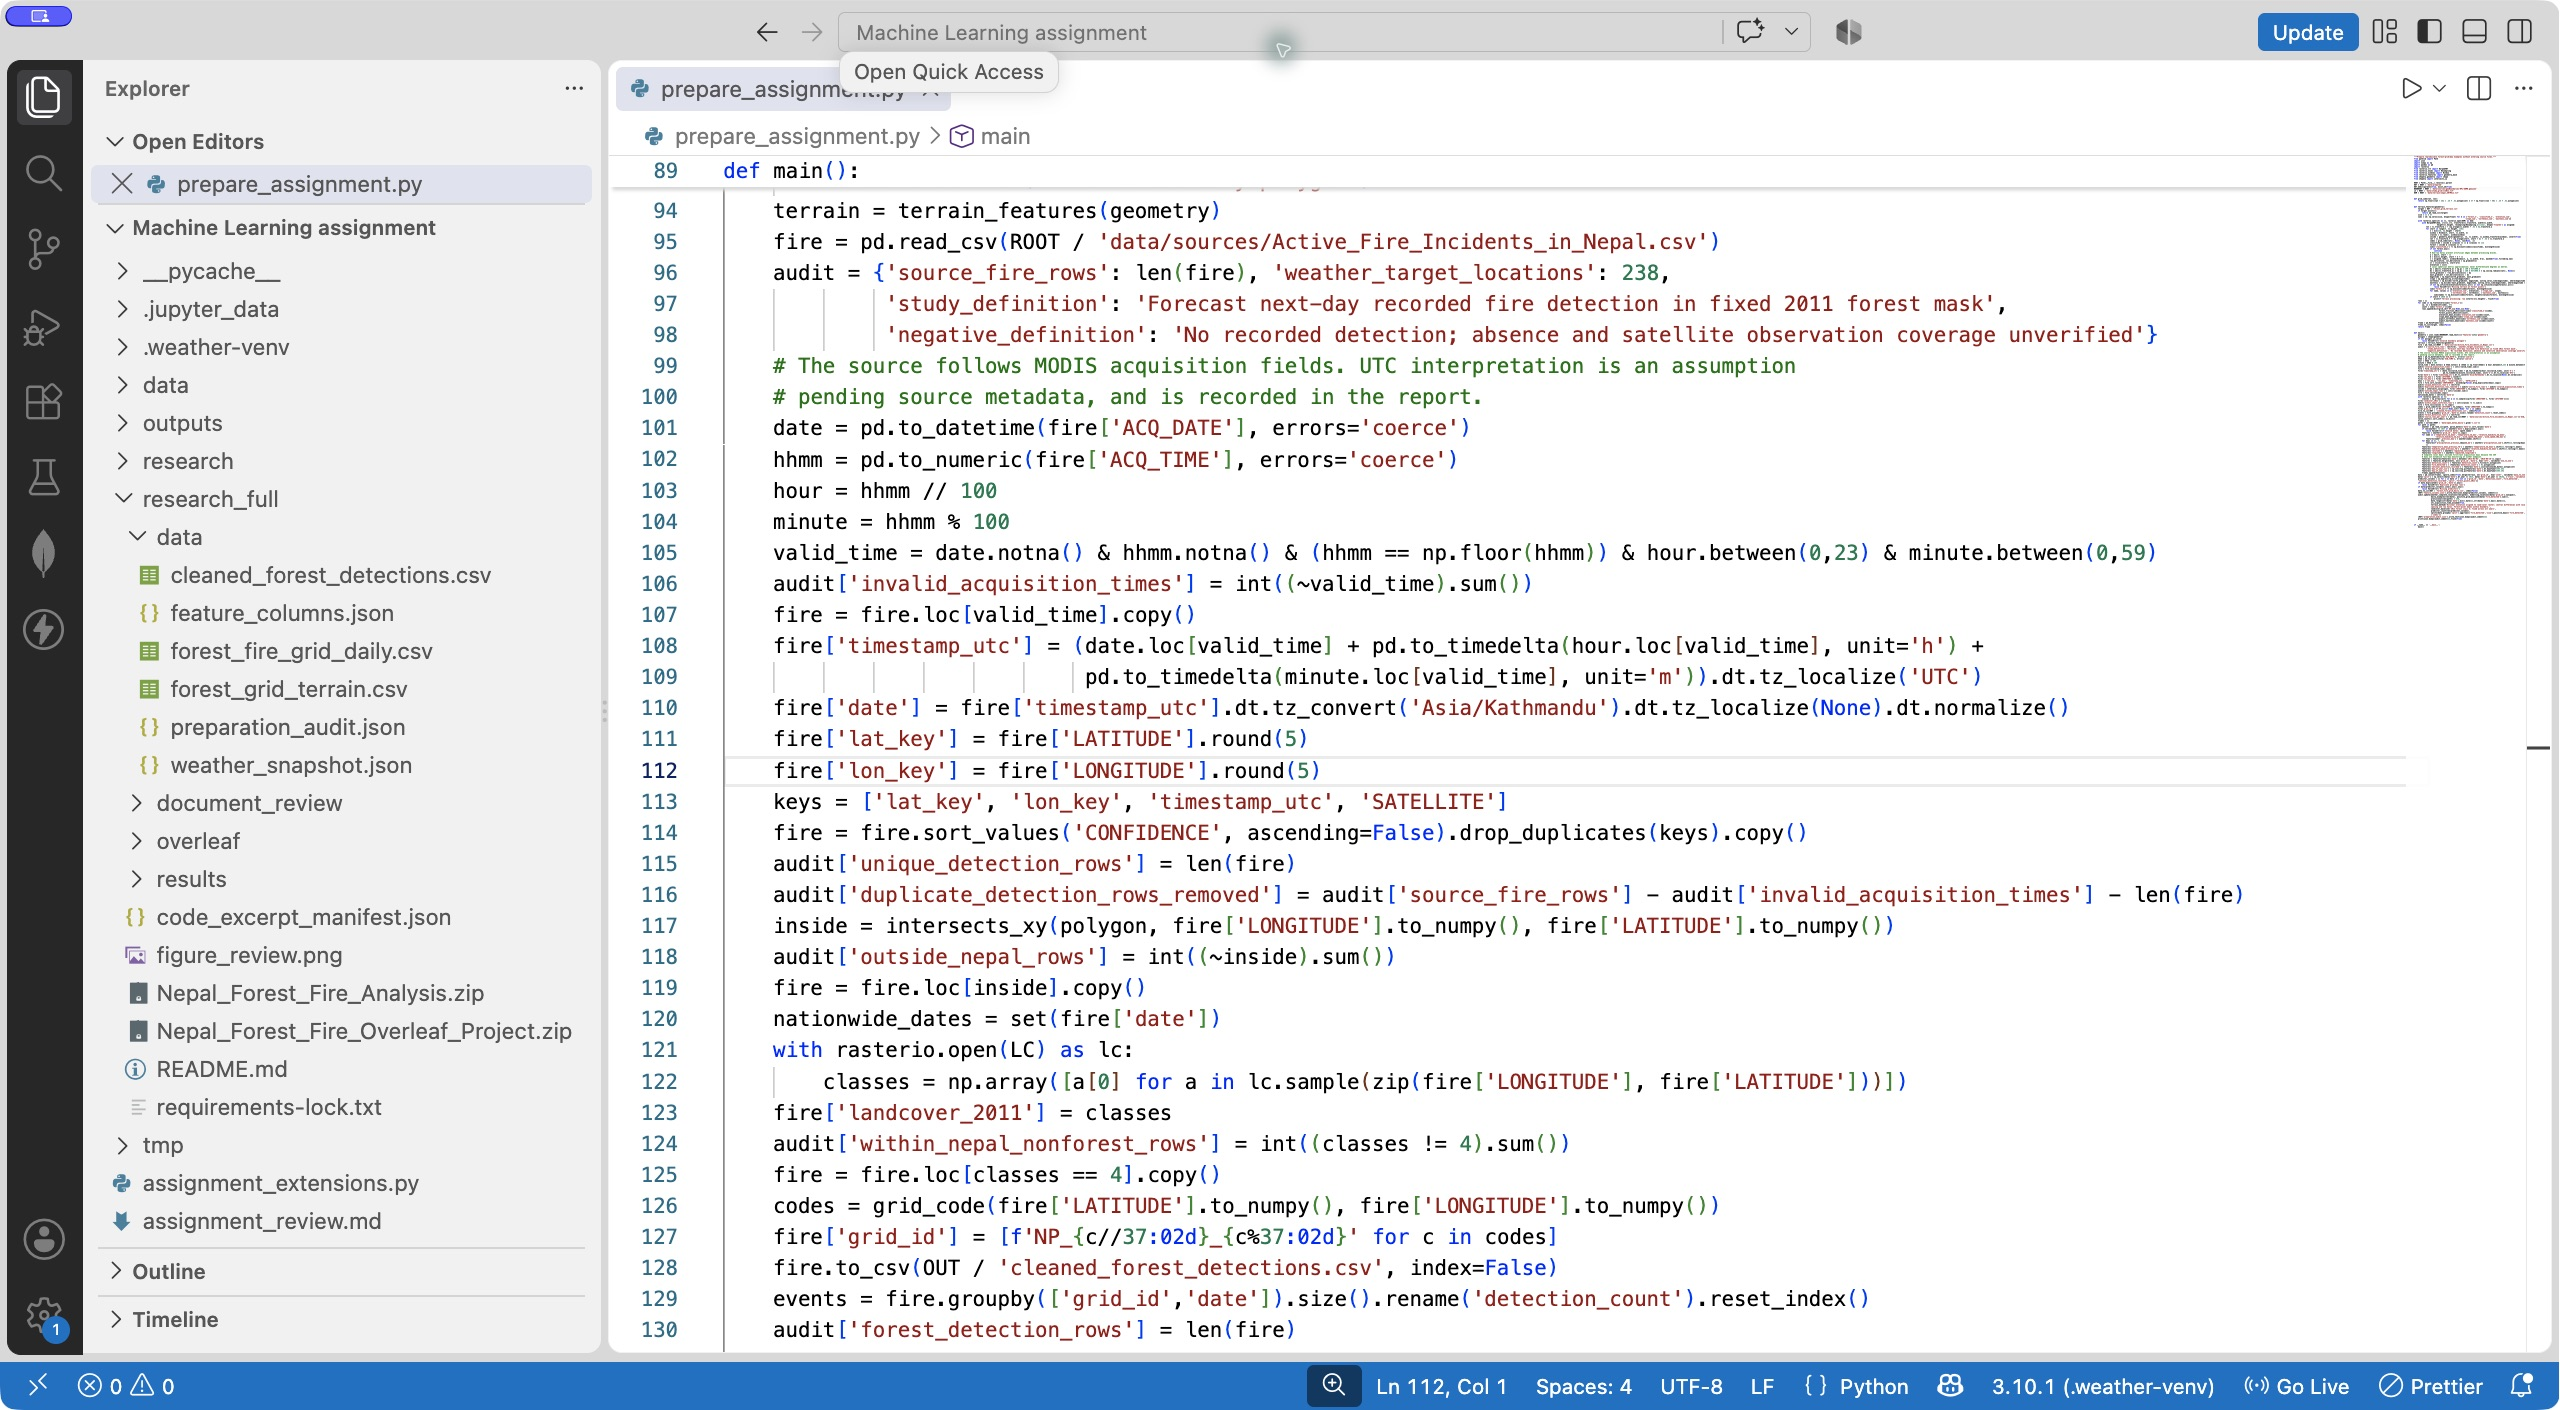
\includegraphics[trim=0 0 0 100,clip,width=\columnwidth]{images/vscode_02_cleaning.png}
\caption{Visual Studio Code: Date conversion, repeated-detection removal and spatial filtering in prepare\_assignment.py.}
\label{fig:appendix-vscode-1}
\end{figure}

\begin{figure}[!htbp]
\centering
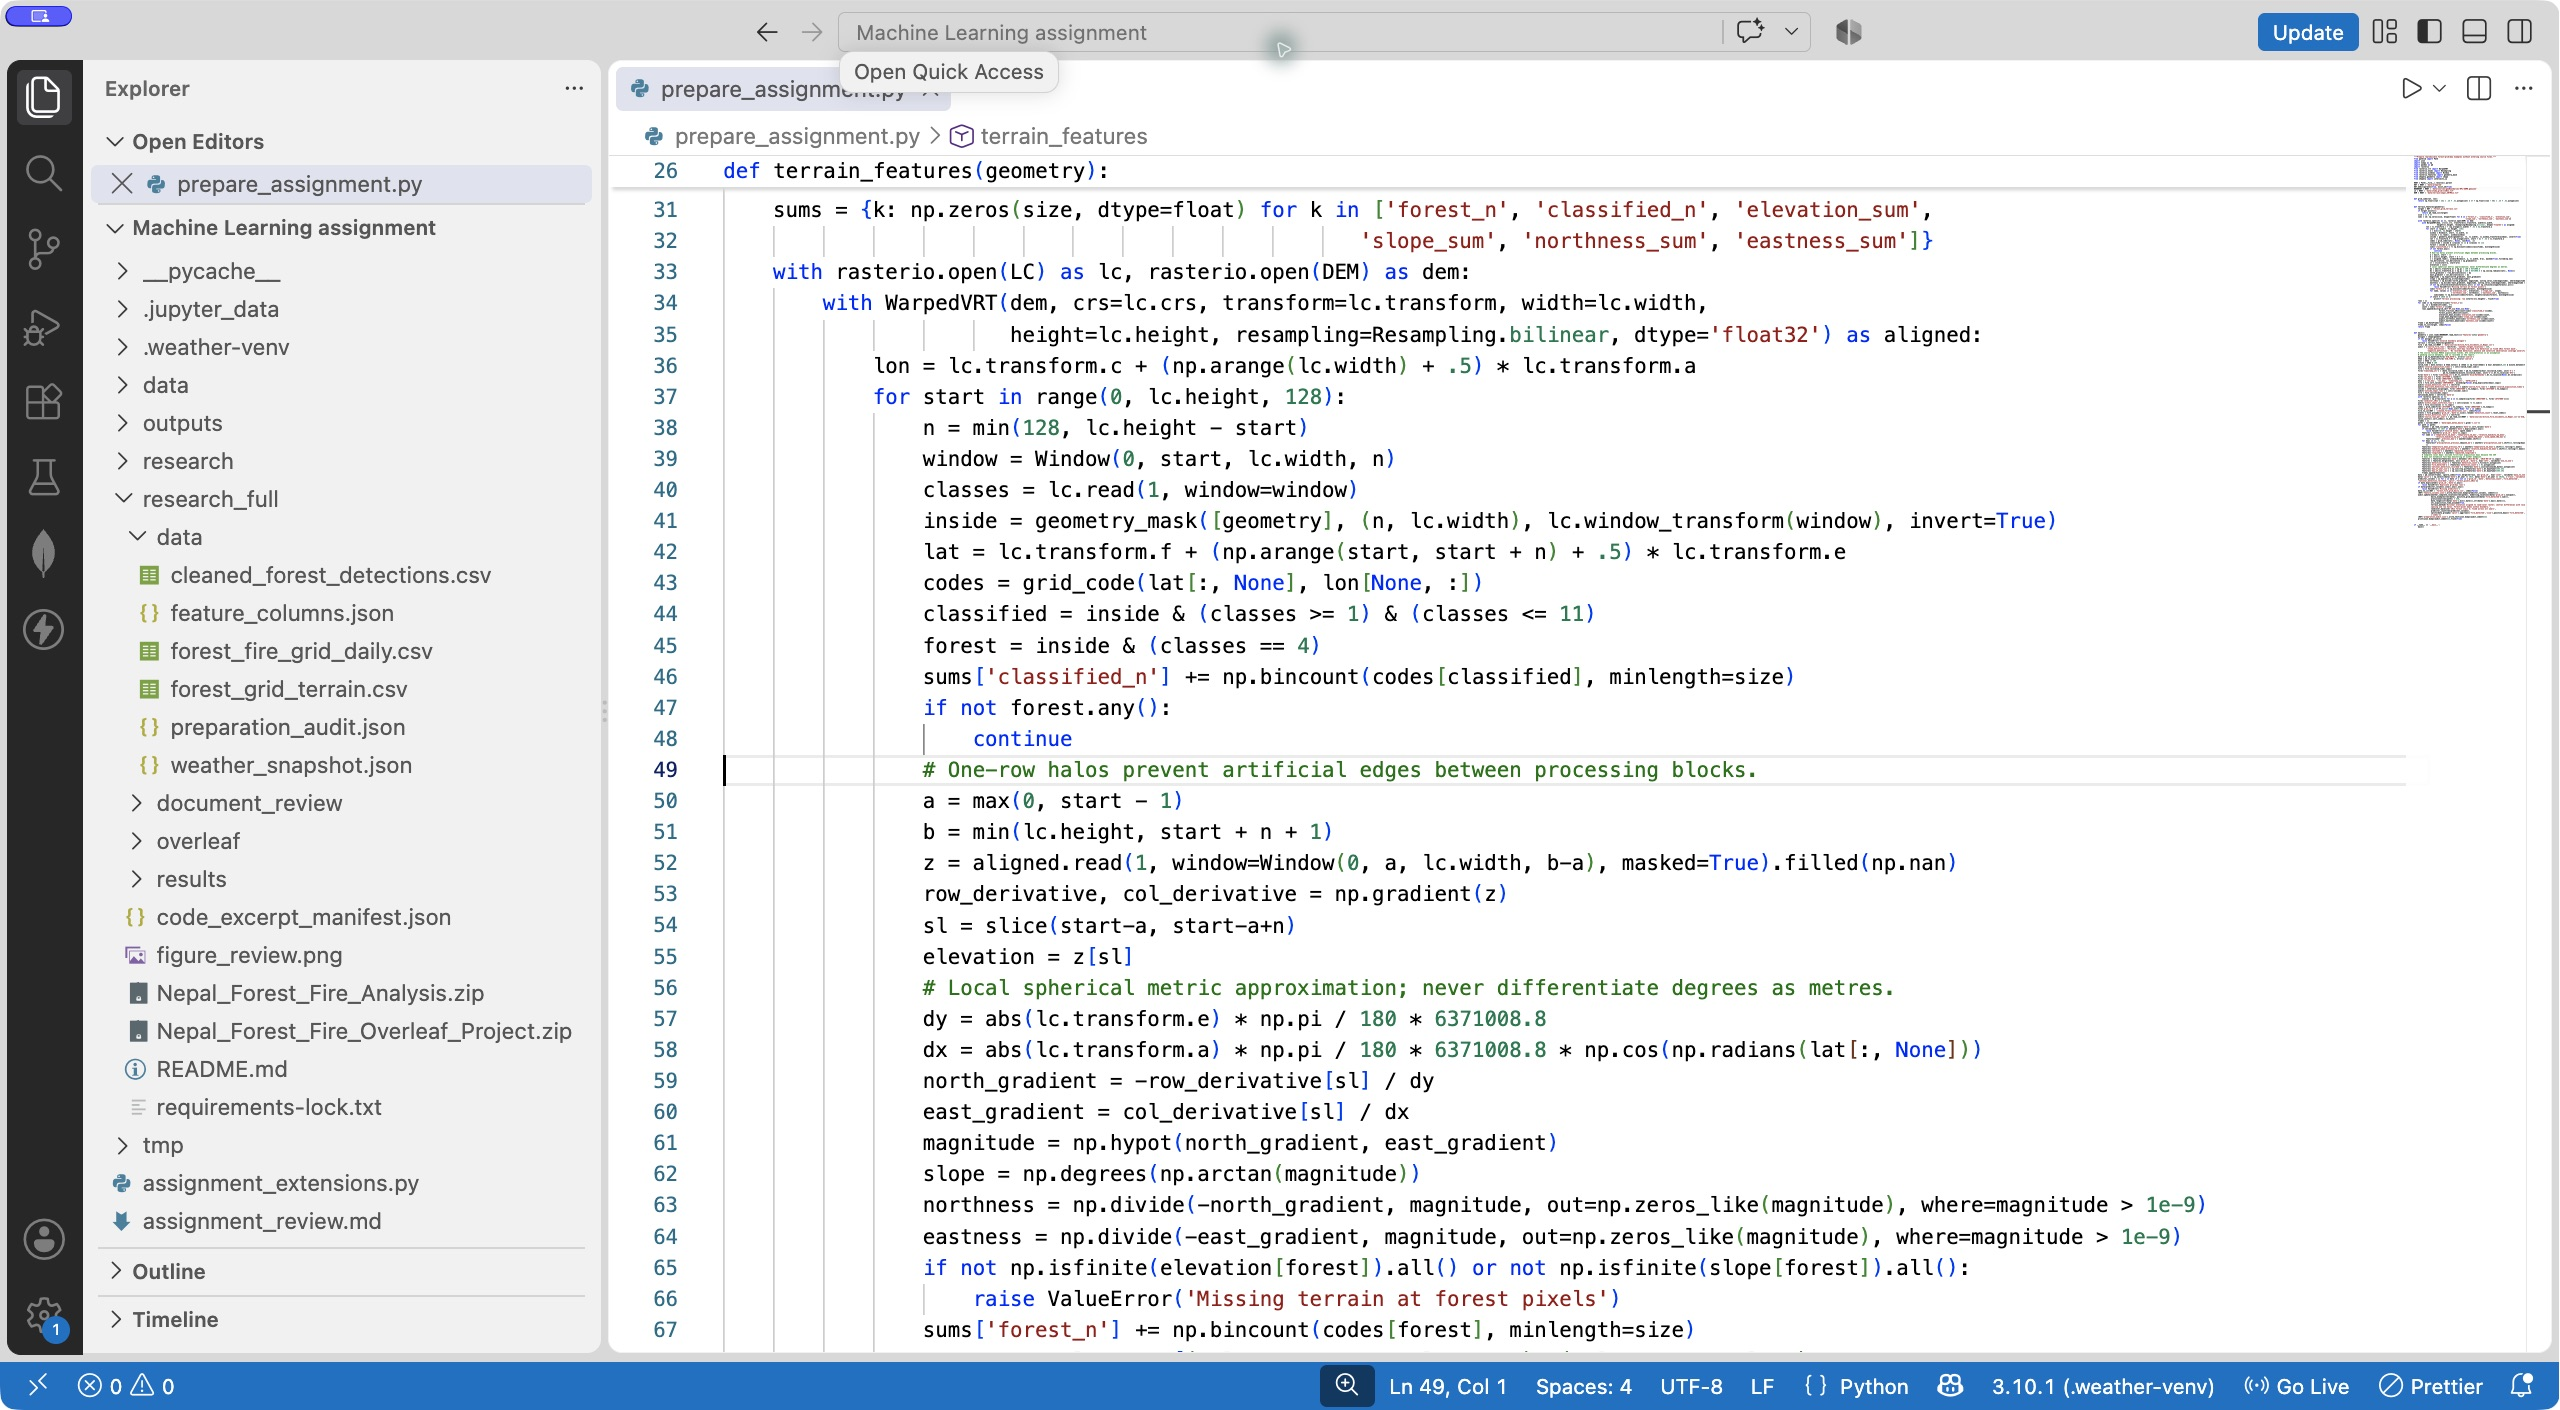
\includegraphics[trim=0 0 0 100,clip,width=\columnwidth]{images/vscode_04_terrain.png}
\caption{Visual Studio Code: Terrain gradients and forest statistics in prepare\_assignment.py.}
\label{fig:appendix-vscode-2}
\end{figure}

\begin{figure}[!htbp]
\centering
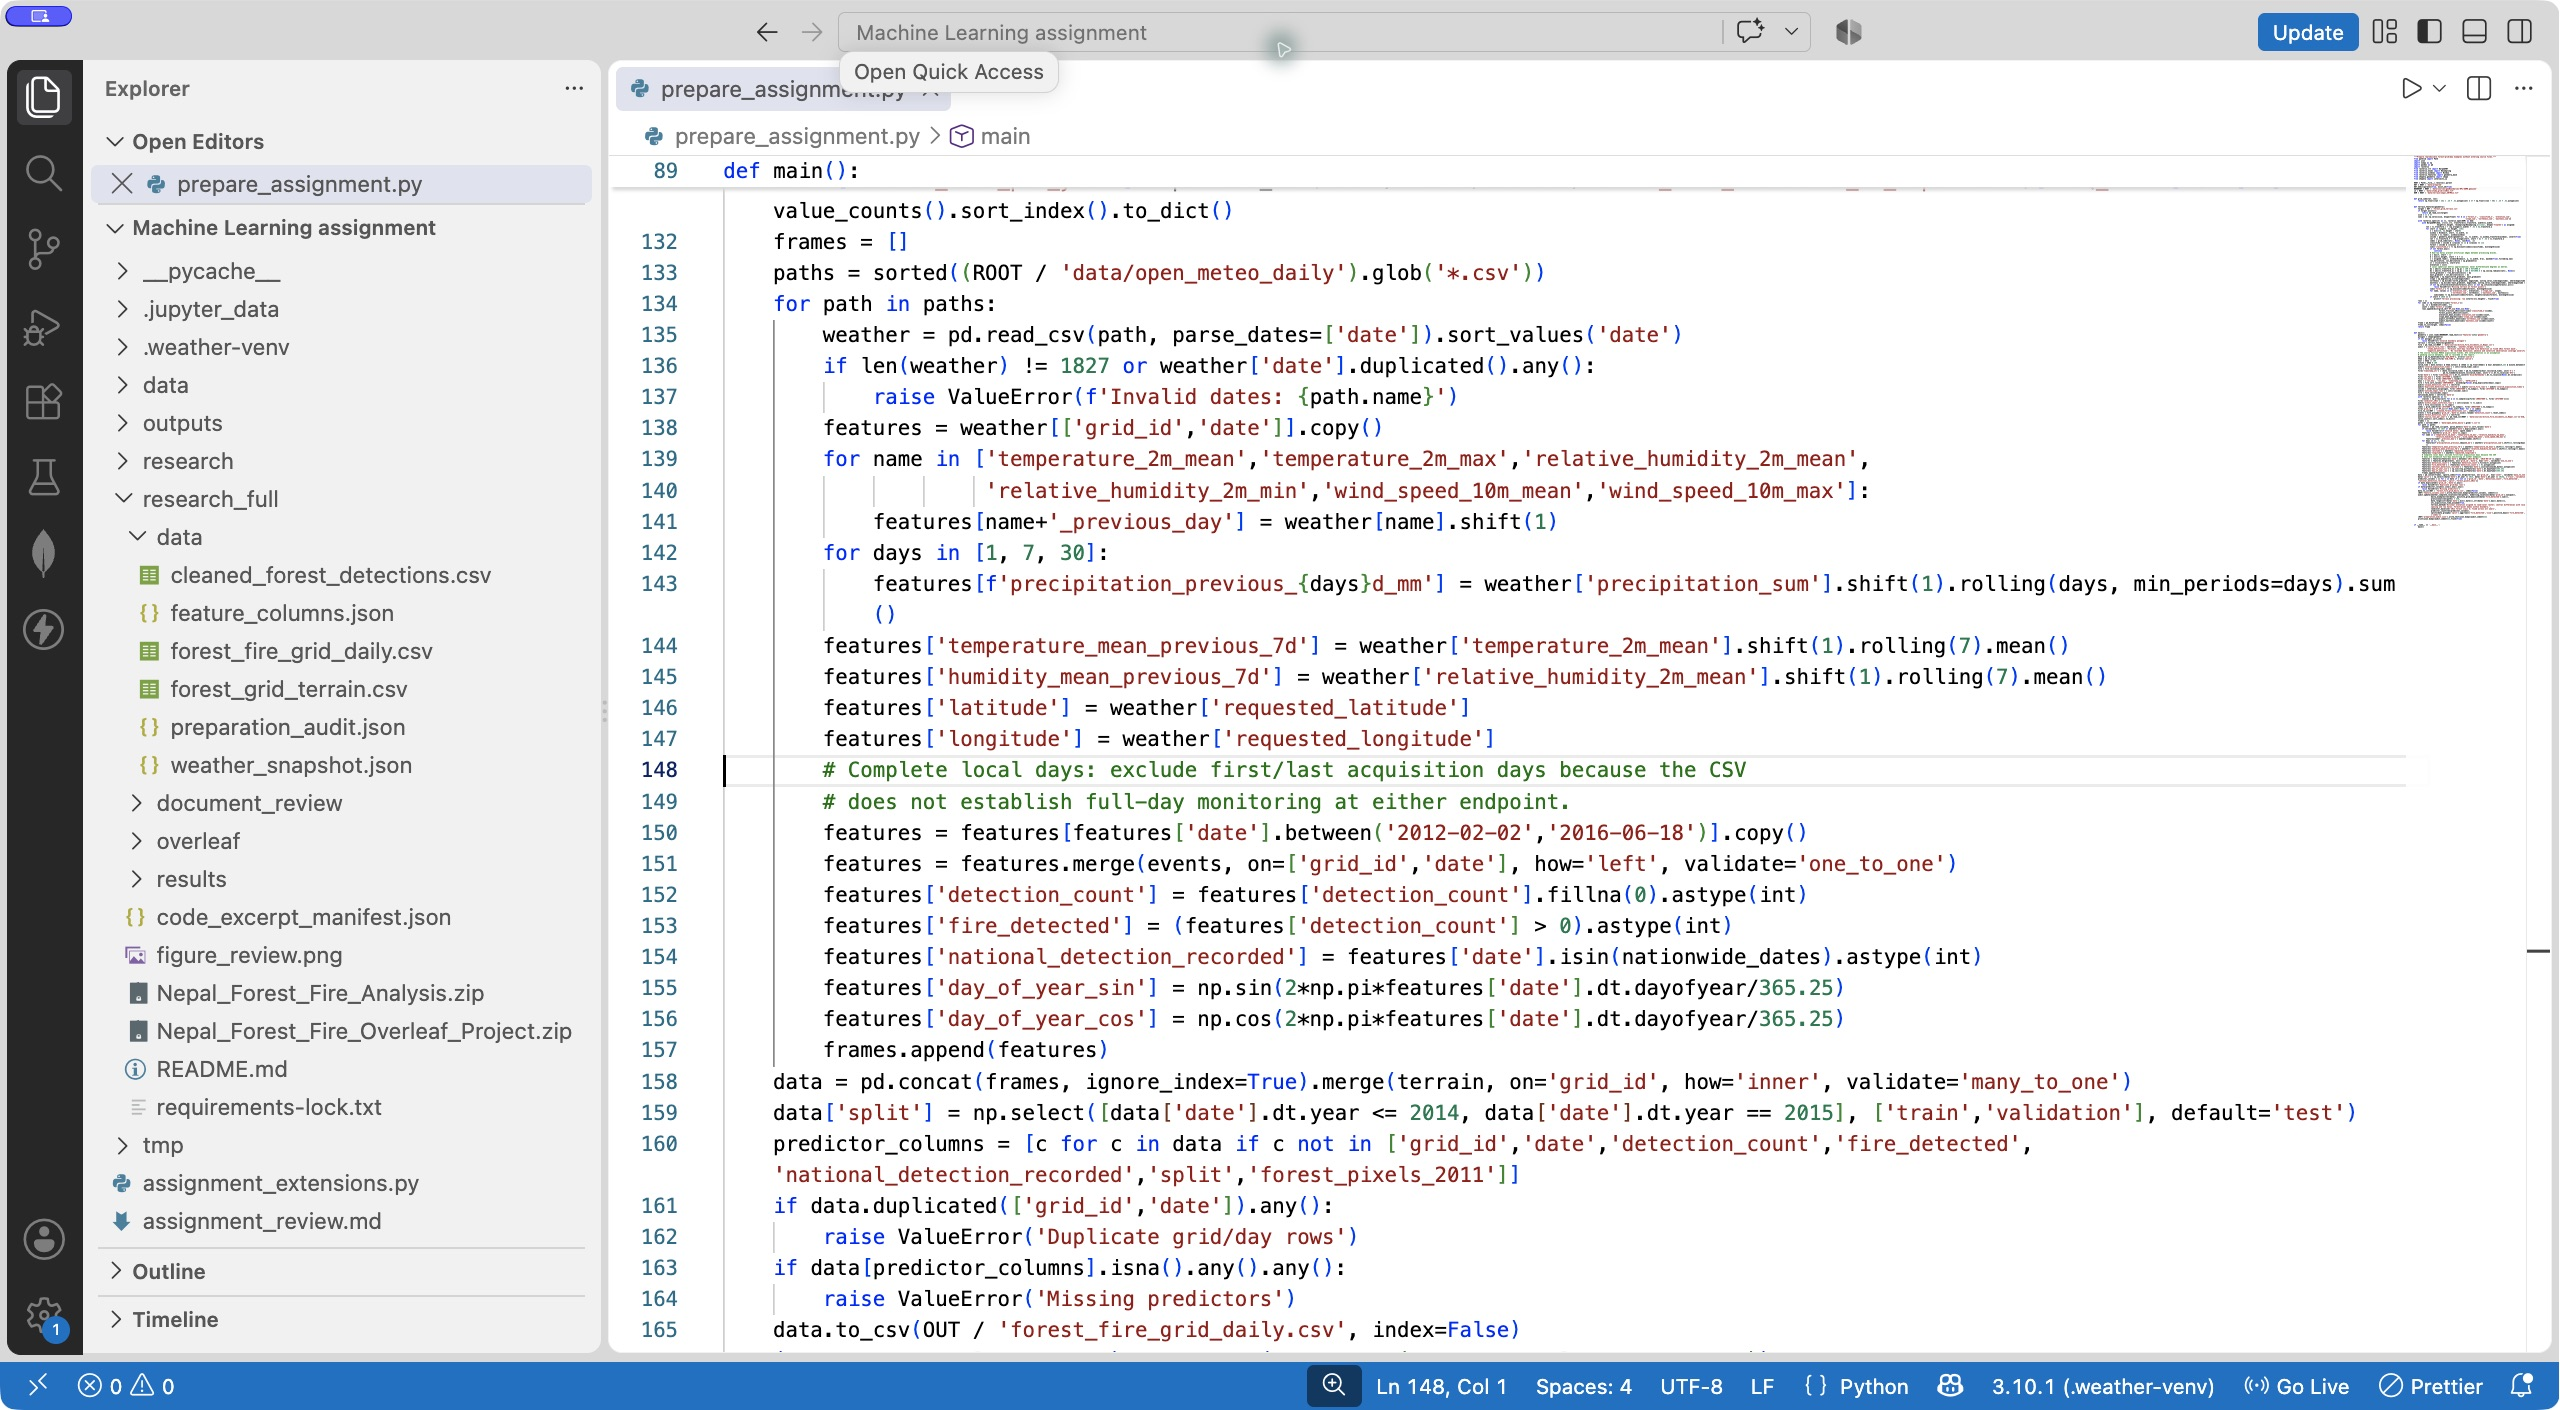
\includegraphics[trim=0 0 0 100,clip,width=\columnwidth]{images/vscode_03_features.png}
\caption{Visual Studio Code: Lagged weather features, rolling summaries and daily target construction in prepare\_assignment.py.}
\label{fig:appendix-vscode-3}
\end{figure}

\begin{figure}[!htbp]
\centering
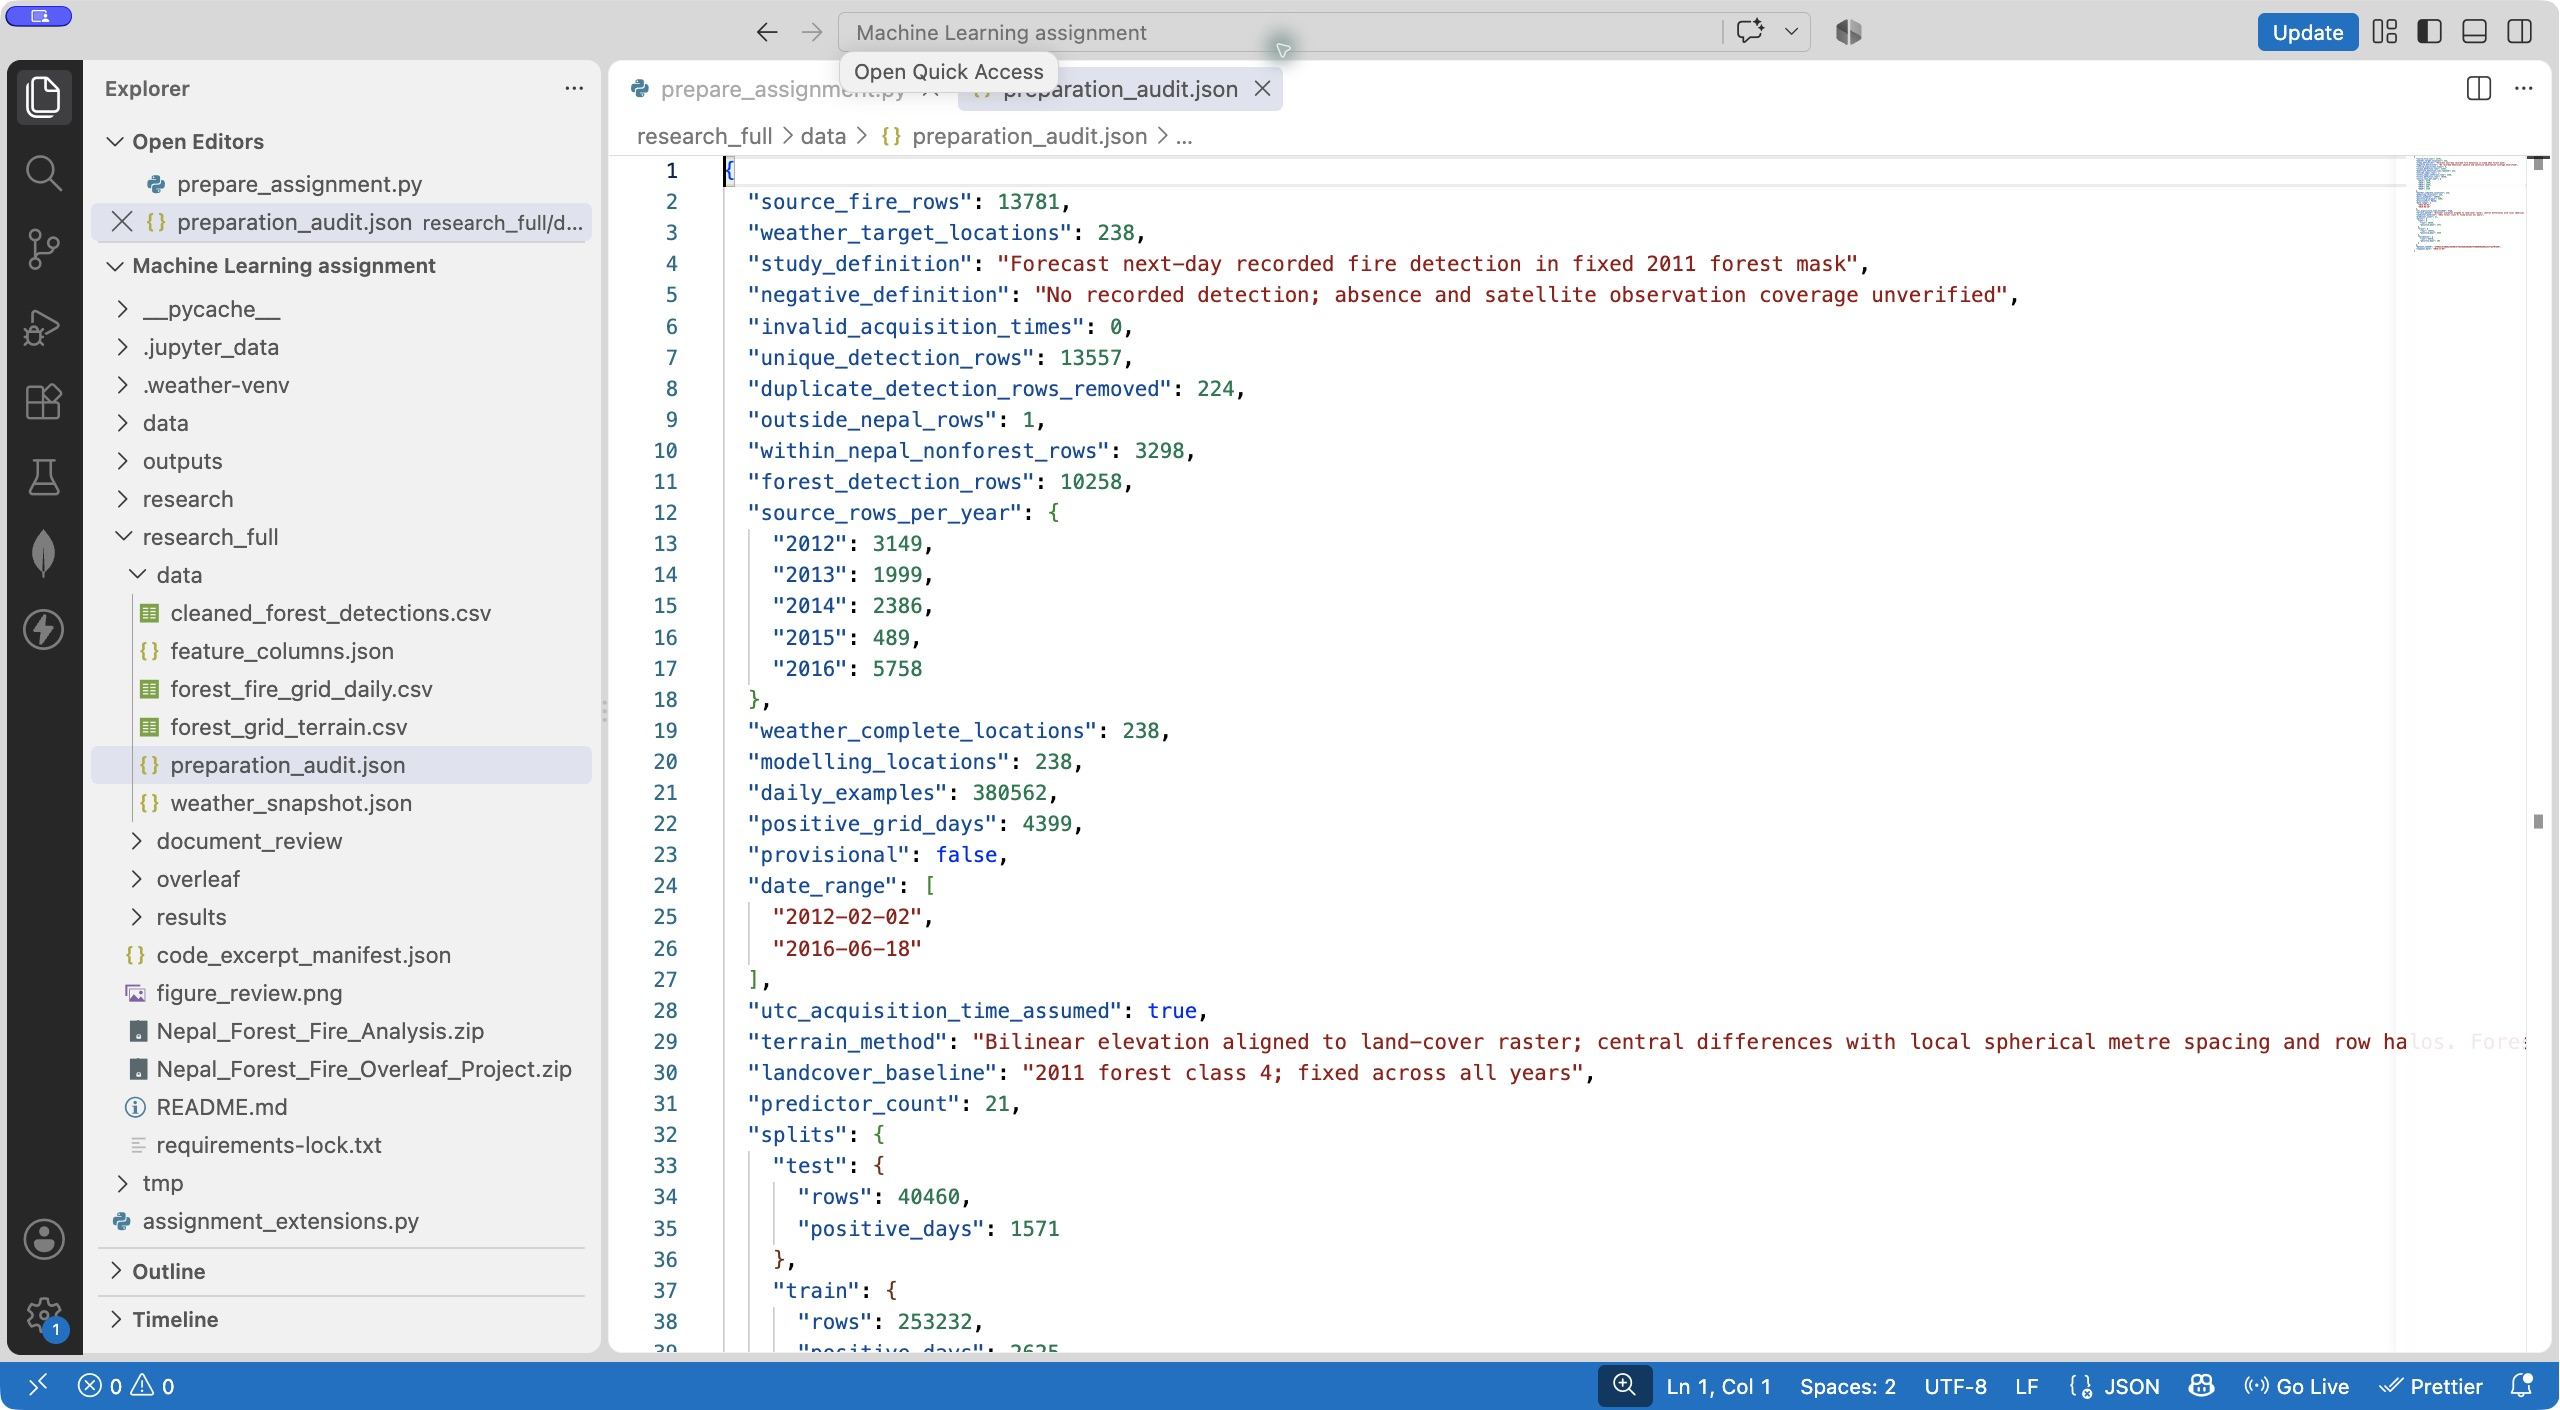
\includegraphics[trim=0 0 0 100,clip,width=\columnwidth]{images/vscode_05_audit.png}
\caption{Visual Studio Code: Saved preparation audit, retained records and chronological data splits.}
\label{fig:appendix-vscode-4}
\end{figure}

\begin{figure}[!htbp]
\centering
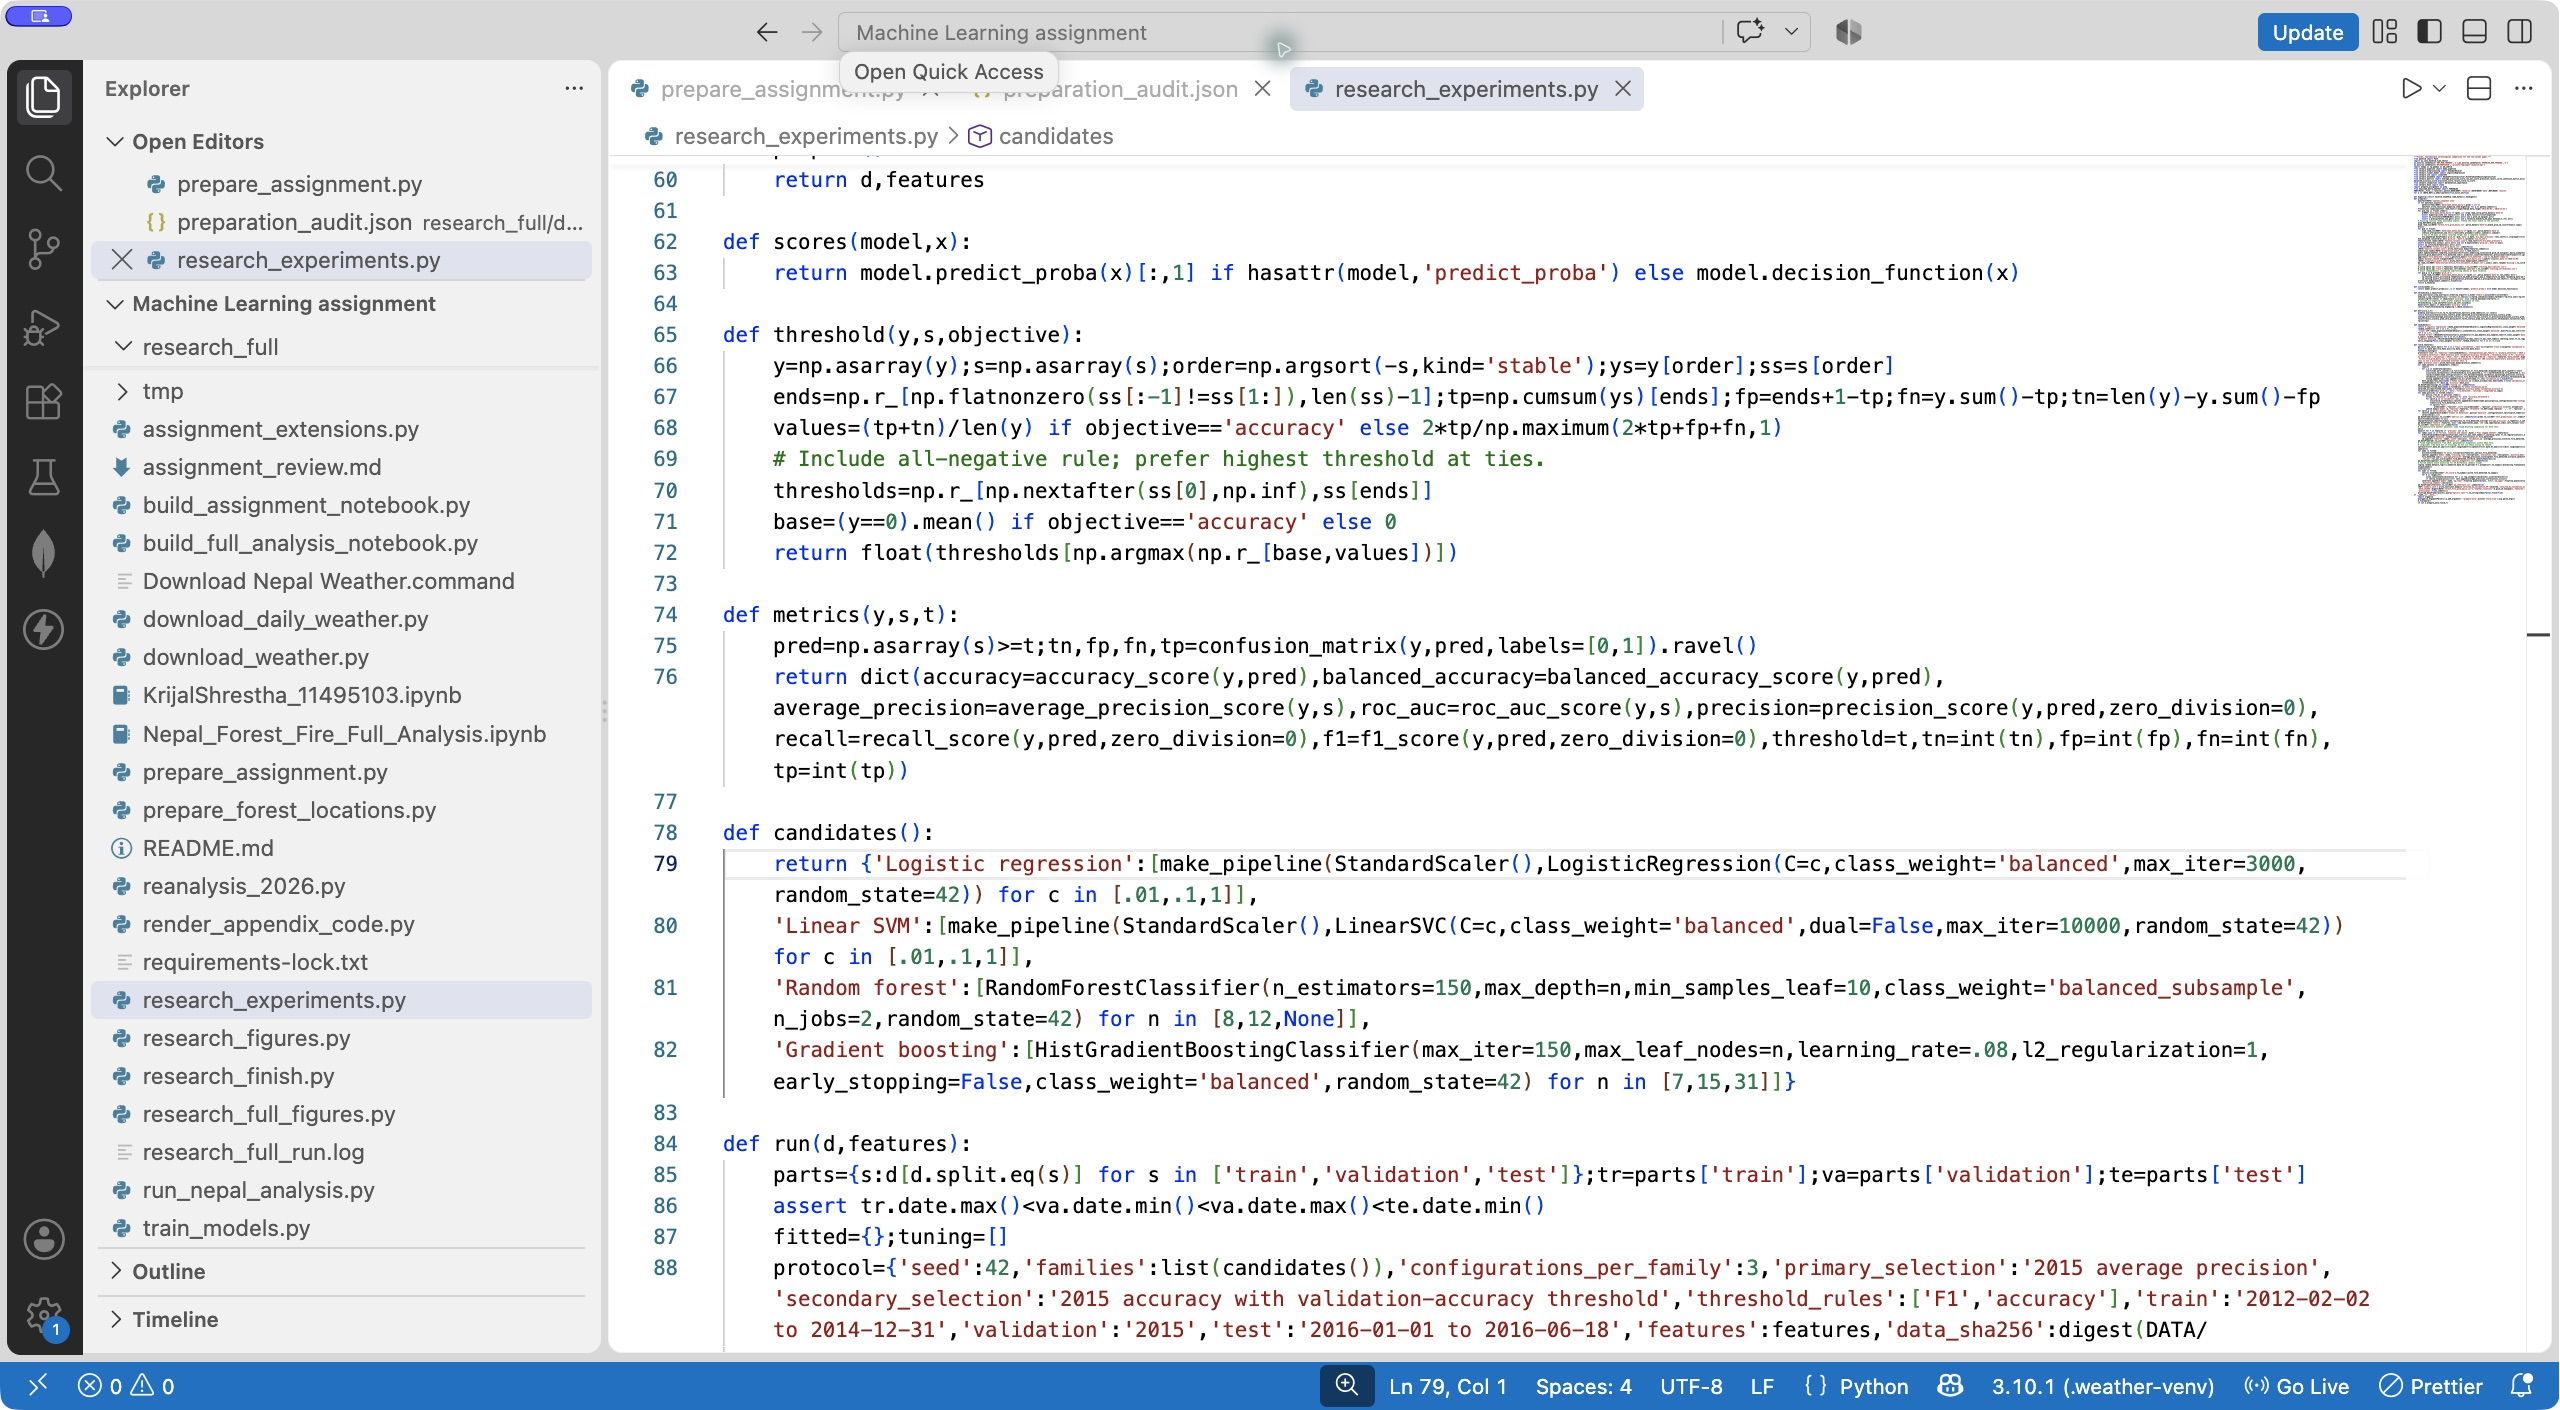
\includegraphics[trim=0 0 0 100,clip,width=\columnwidth]{images/vscode_06_models.png}
\caption{Visual Studio Code: Candidate algorithms, hyperparameters and evaluation helpers in research\_experiments.py.}
\label{fig:appendix-vscode-5}
\end{figure}

\begin{figure}[!htbp]
\centering
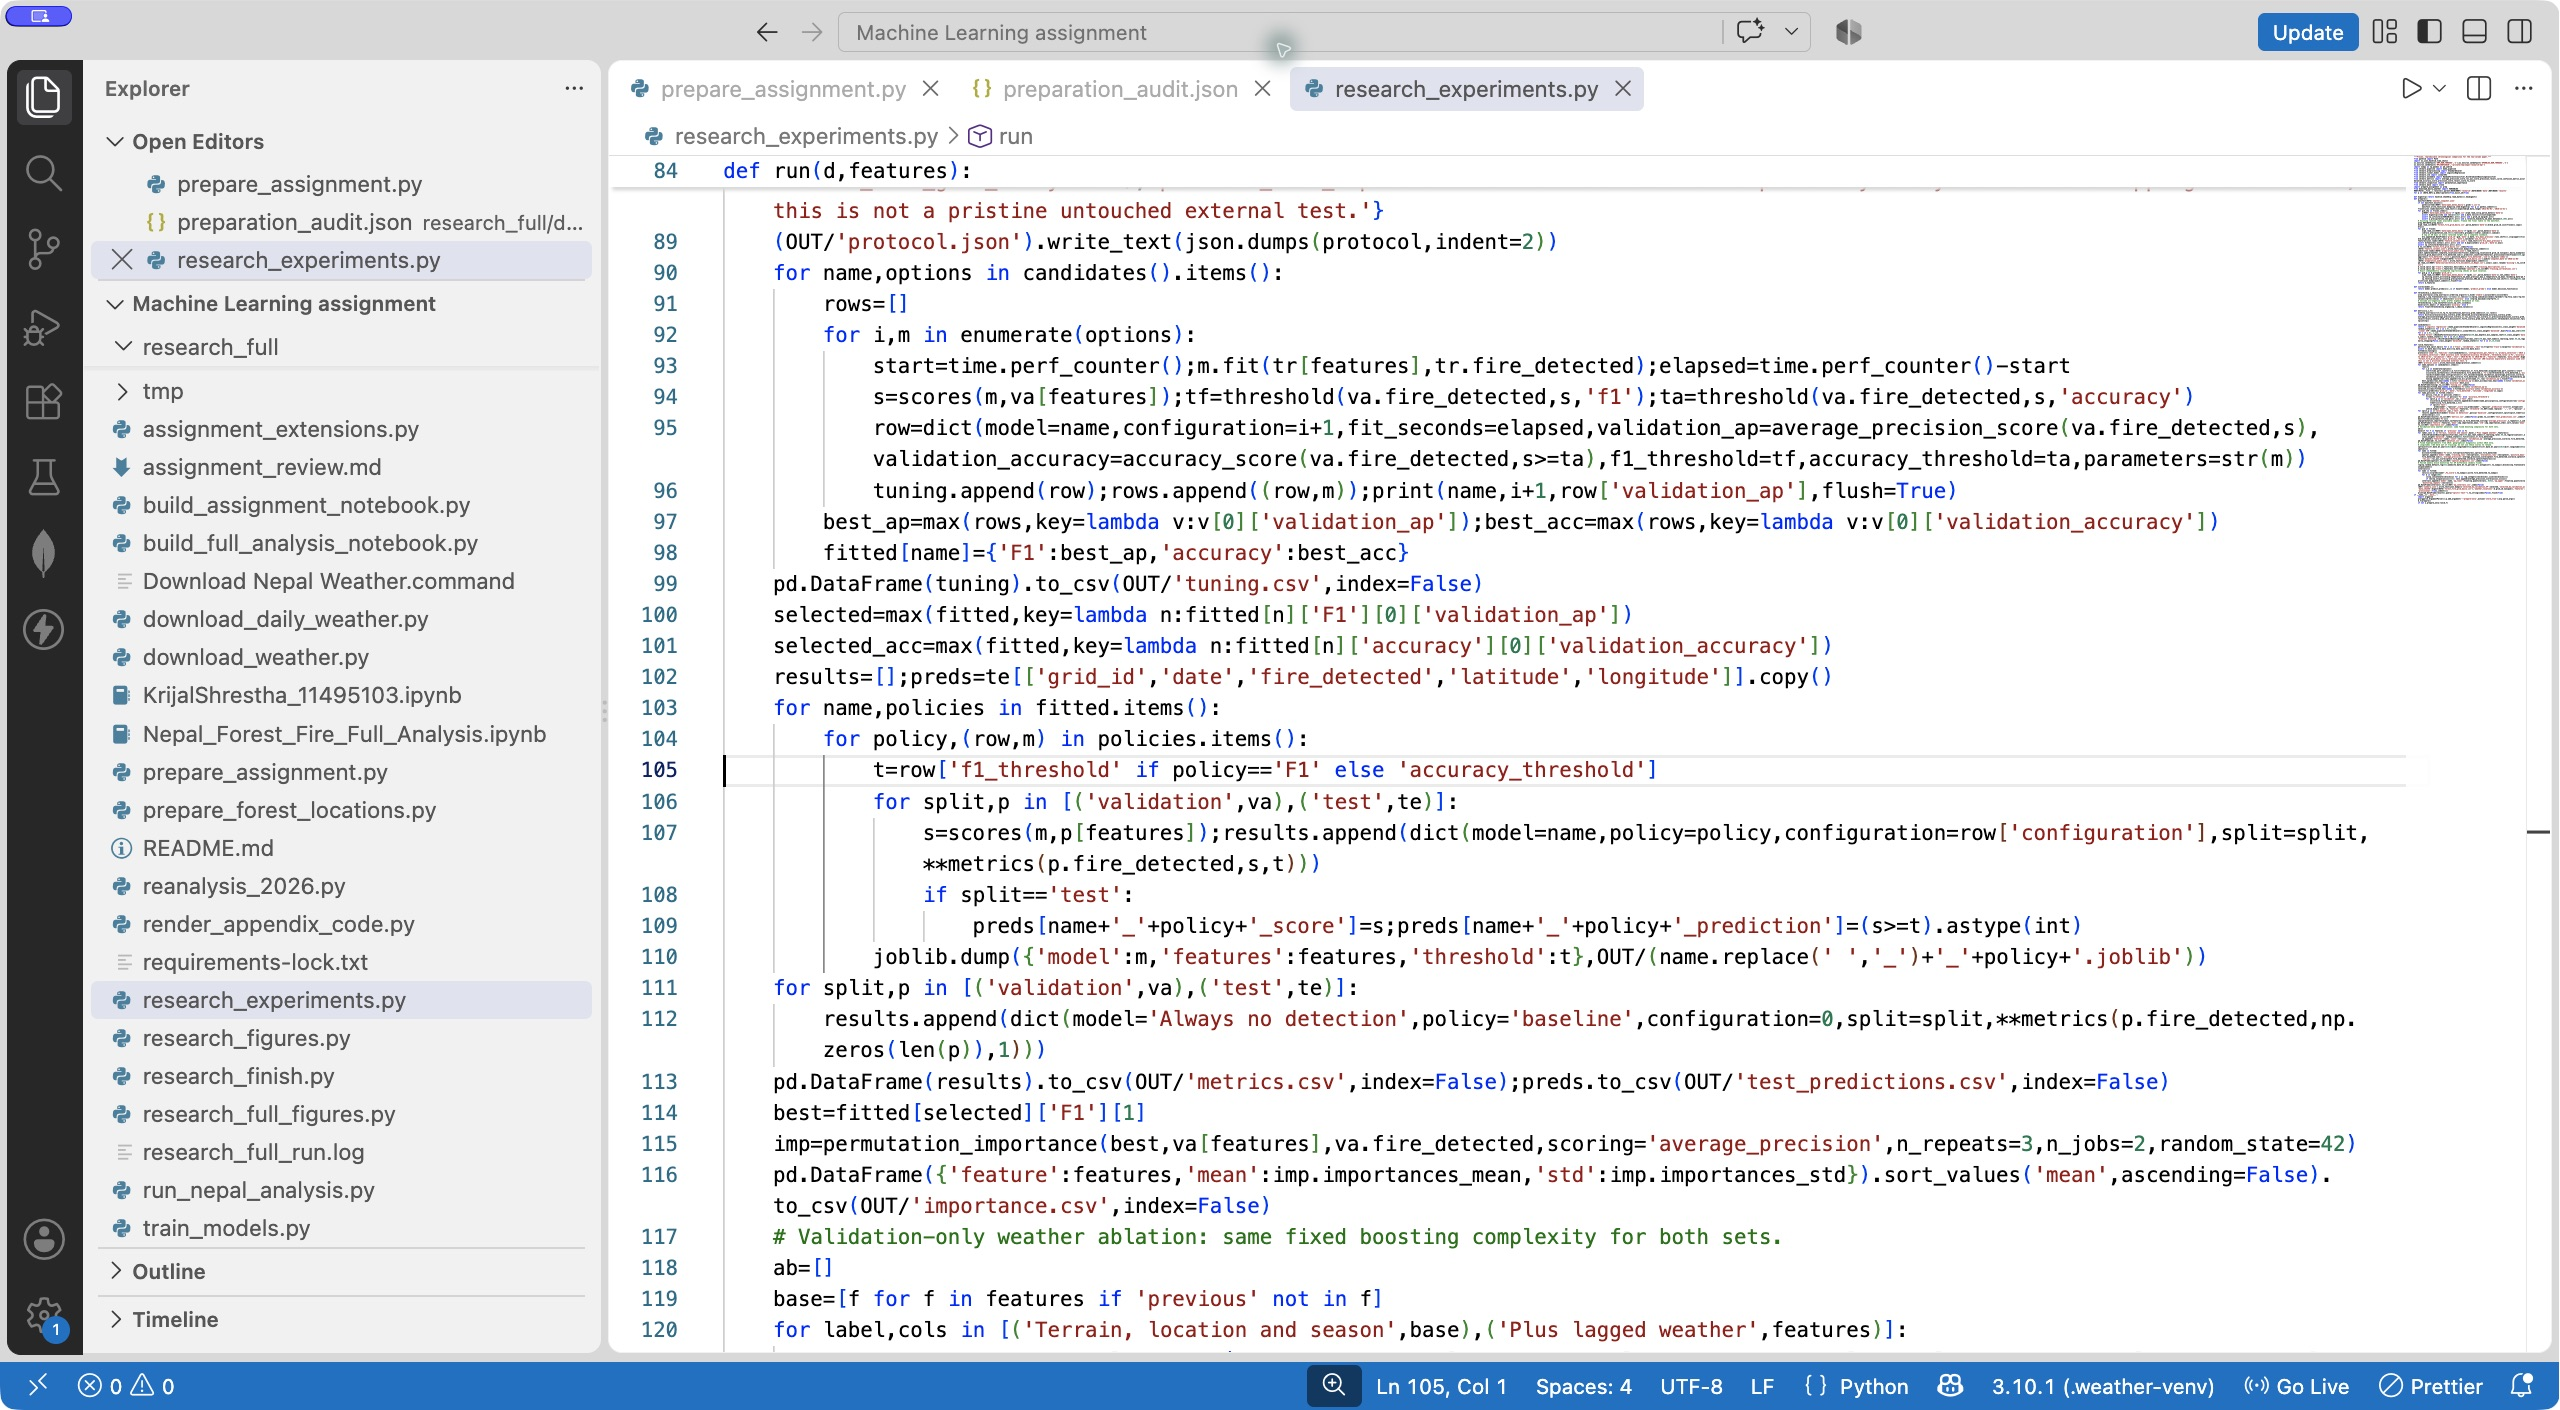
\includegraphics[trim=0 0 0 100,clip,width=\columnwidth]{images/vscode_07_training.png}
\caption{Visual Studio Code: Candidate fitting, validation selection and saved evaluation outputs in research\_experiments.py.}
\label{fig:appendix-vscode-6}
\end{figure}

\begin{figure}[!htbp]
\centering
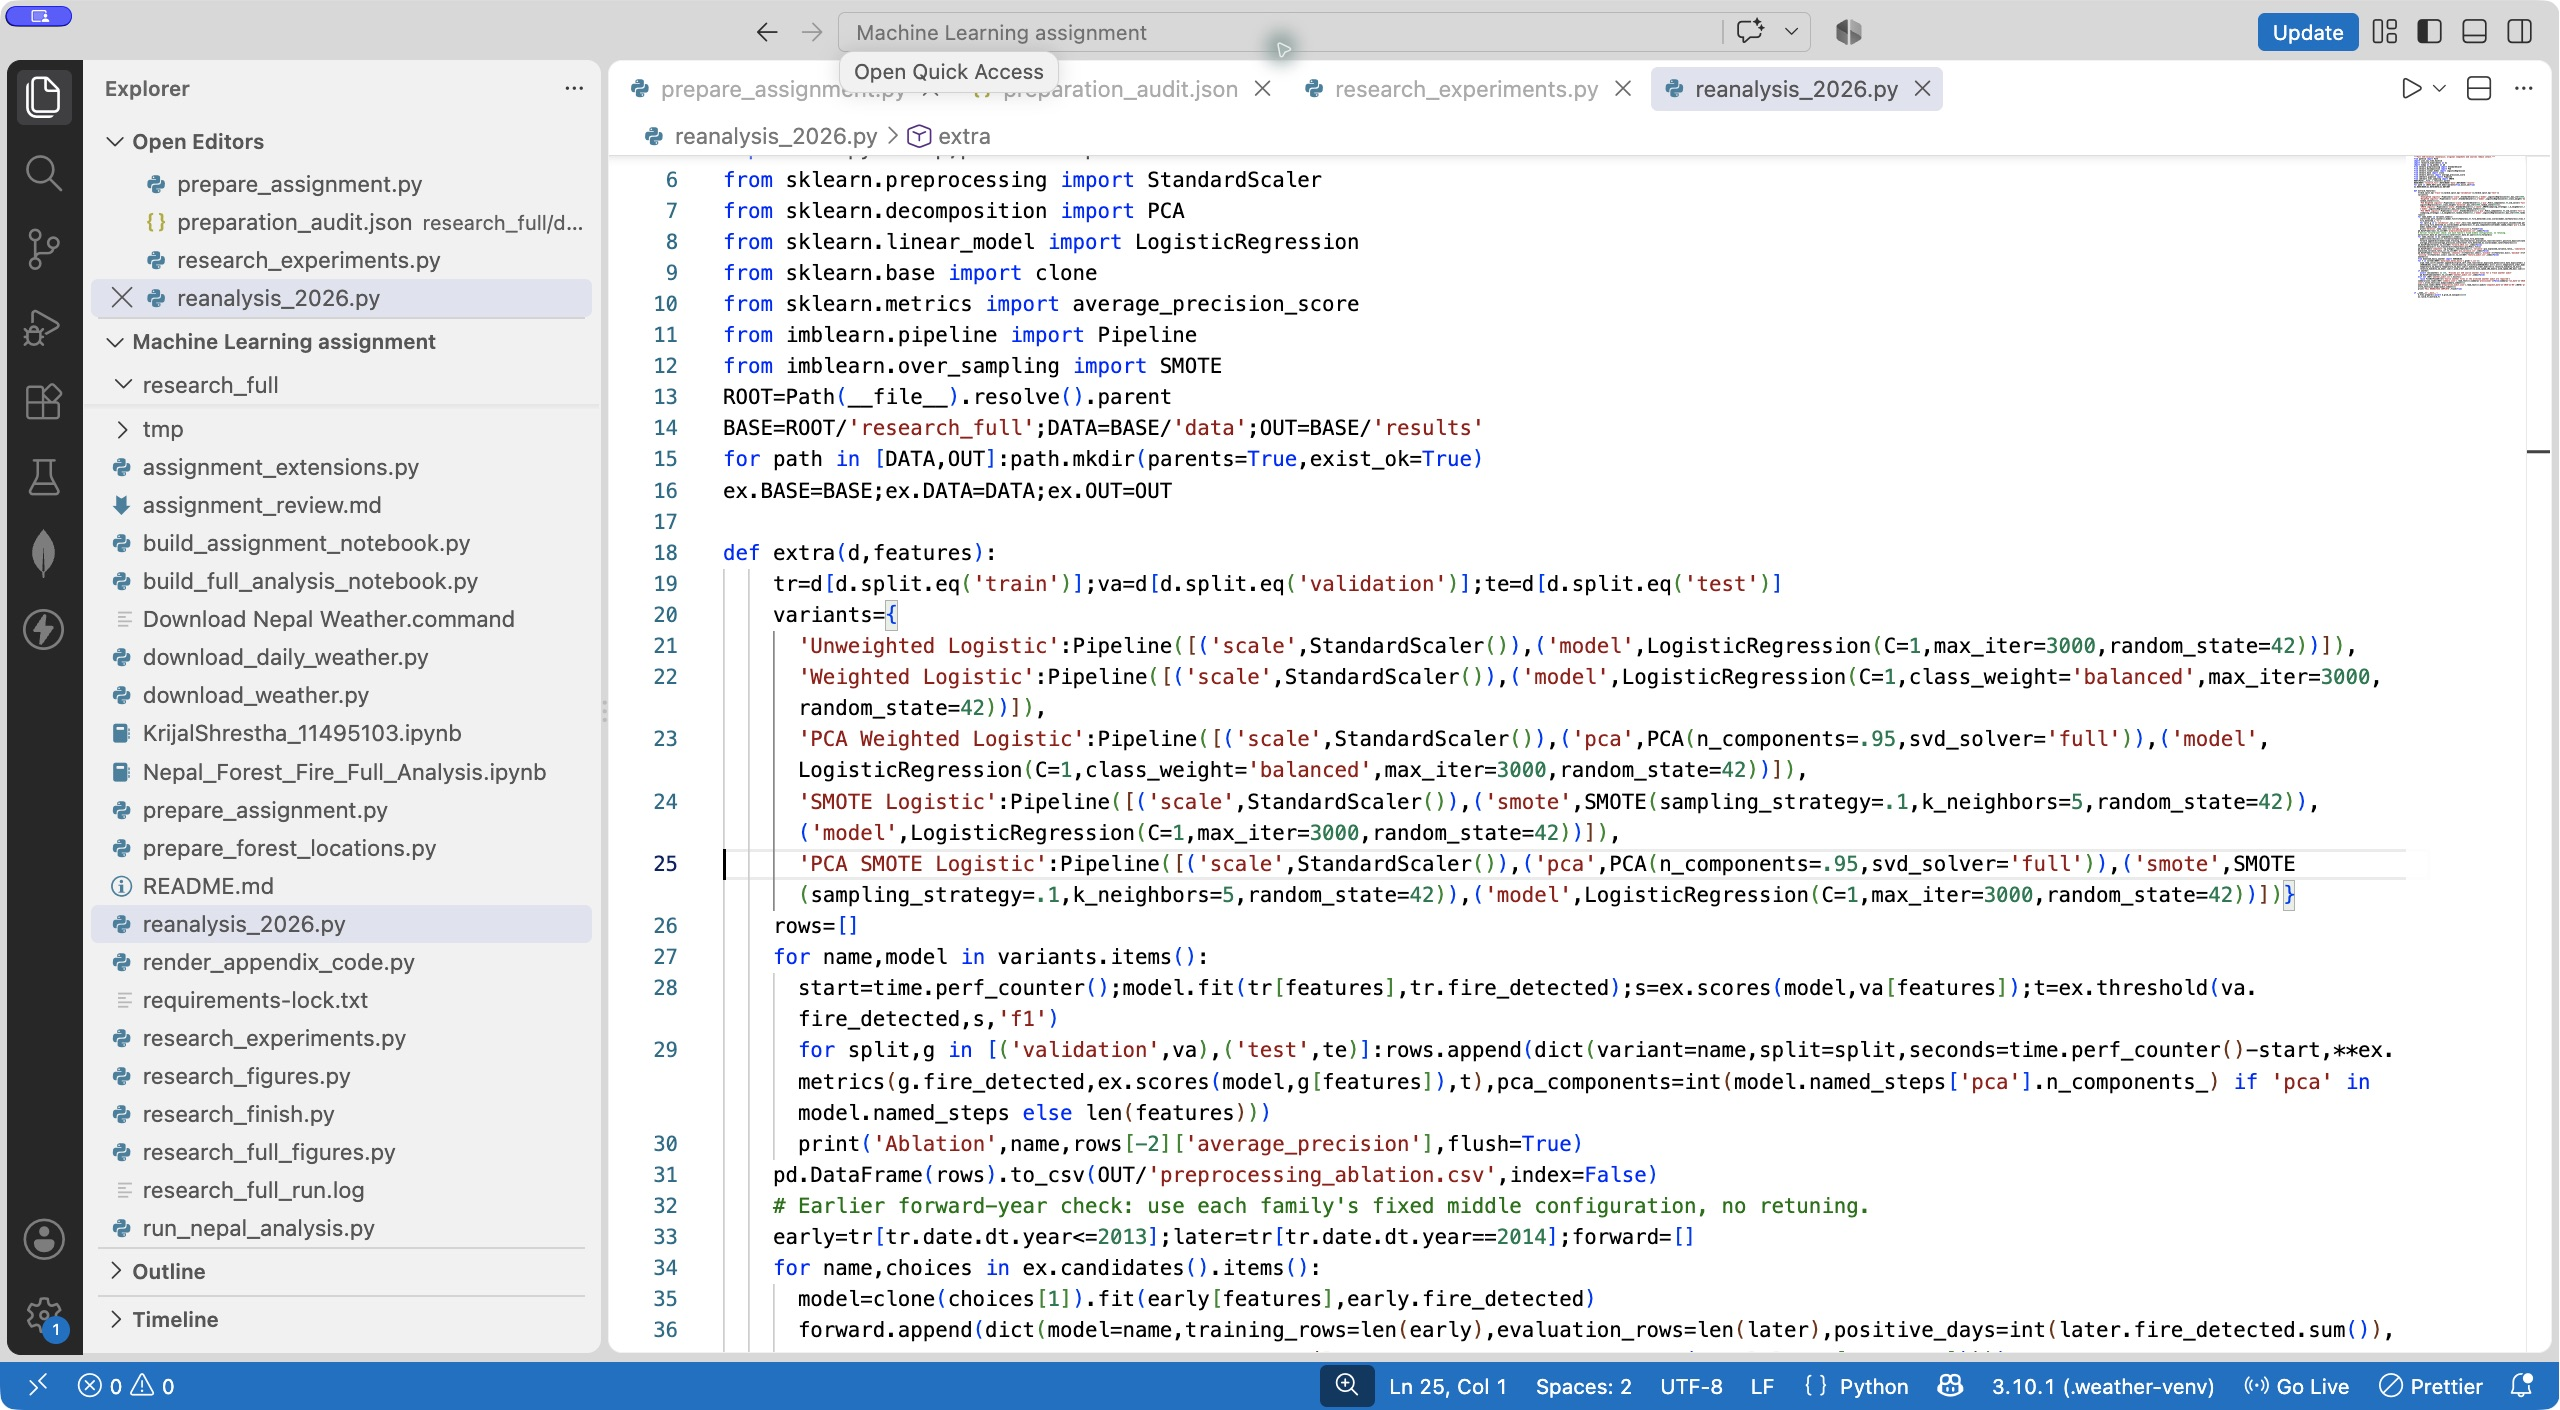
\includegraphics[trim=0 0 0 100,clip,width=\columnwidth]{images/vscode_08_preprocessing.png}
\caption{Visual Studio Code: Controlled scaling, class-weighting, PCA and SMOTE comparisons in reanalysis\_2026.py.}
\label{fig:appendix-vscode-7}
\end{figure}

\begin{figure}[!htbp]
\centering
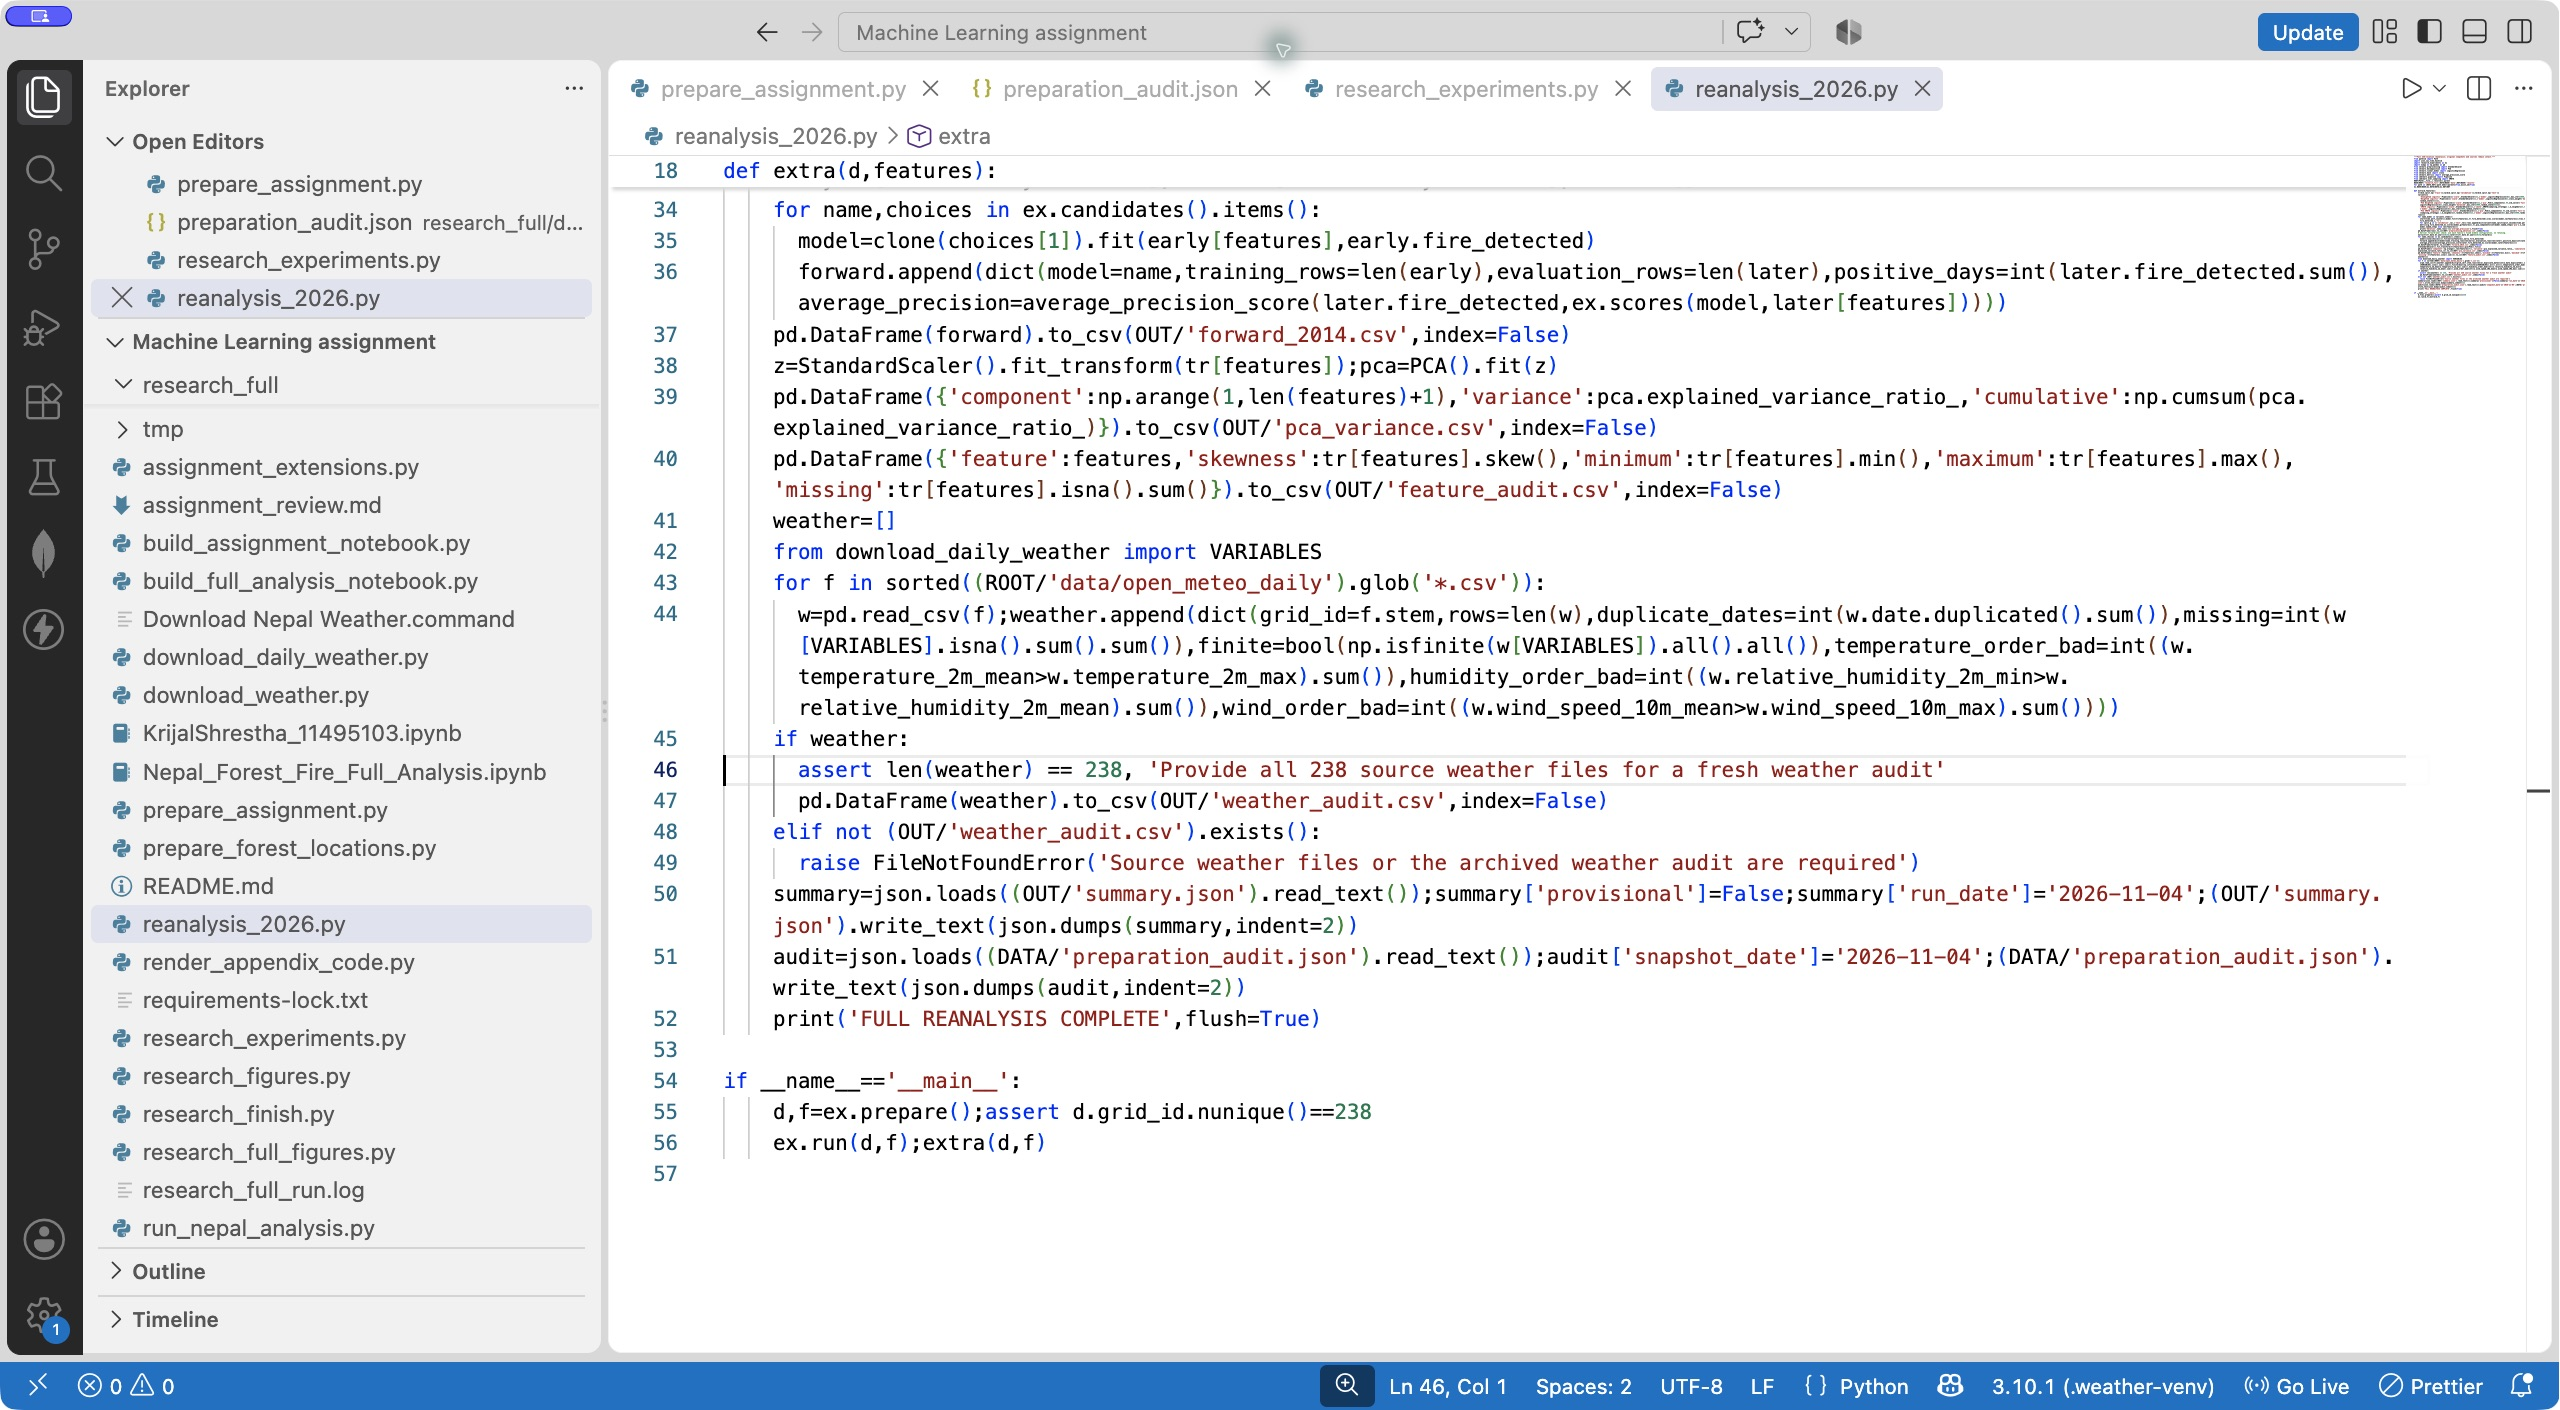
\includegraphics[trim=0 0 0 100,clip,width=\columnwidth]{images/vscode_09_checks.png}
\caption{Visual Studio Code: Additional evaluation checks and weather-data assertions in reanalysis\_2026.py.}
\label{fig:appendix-vscode-8}
\end{figure}

\begin{figure}[!htbp]
\centering
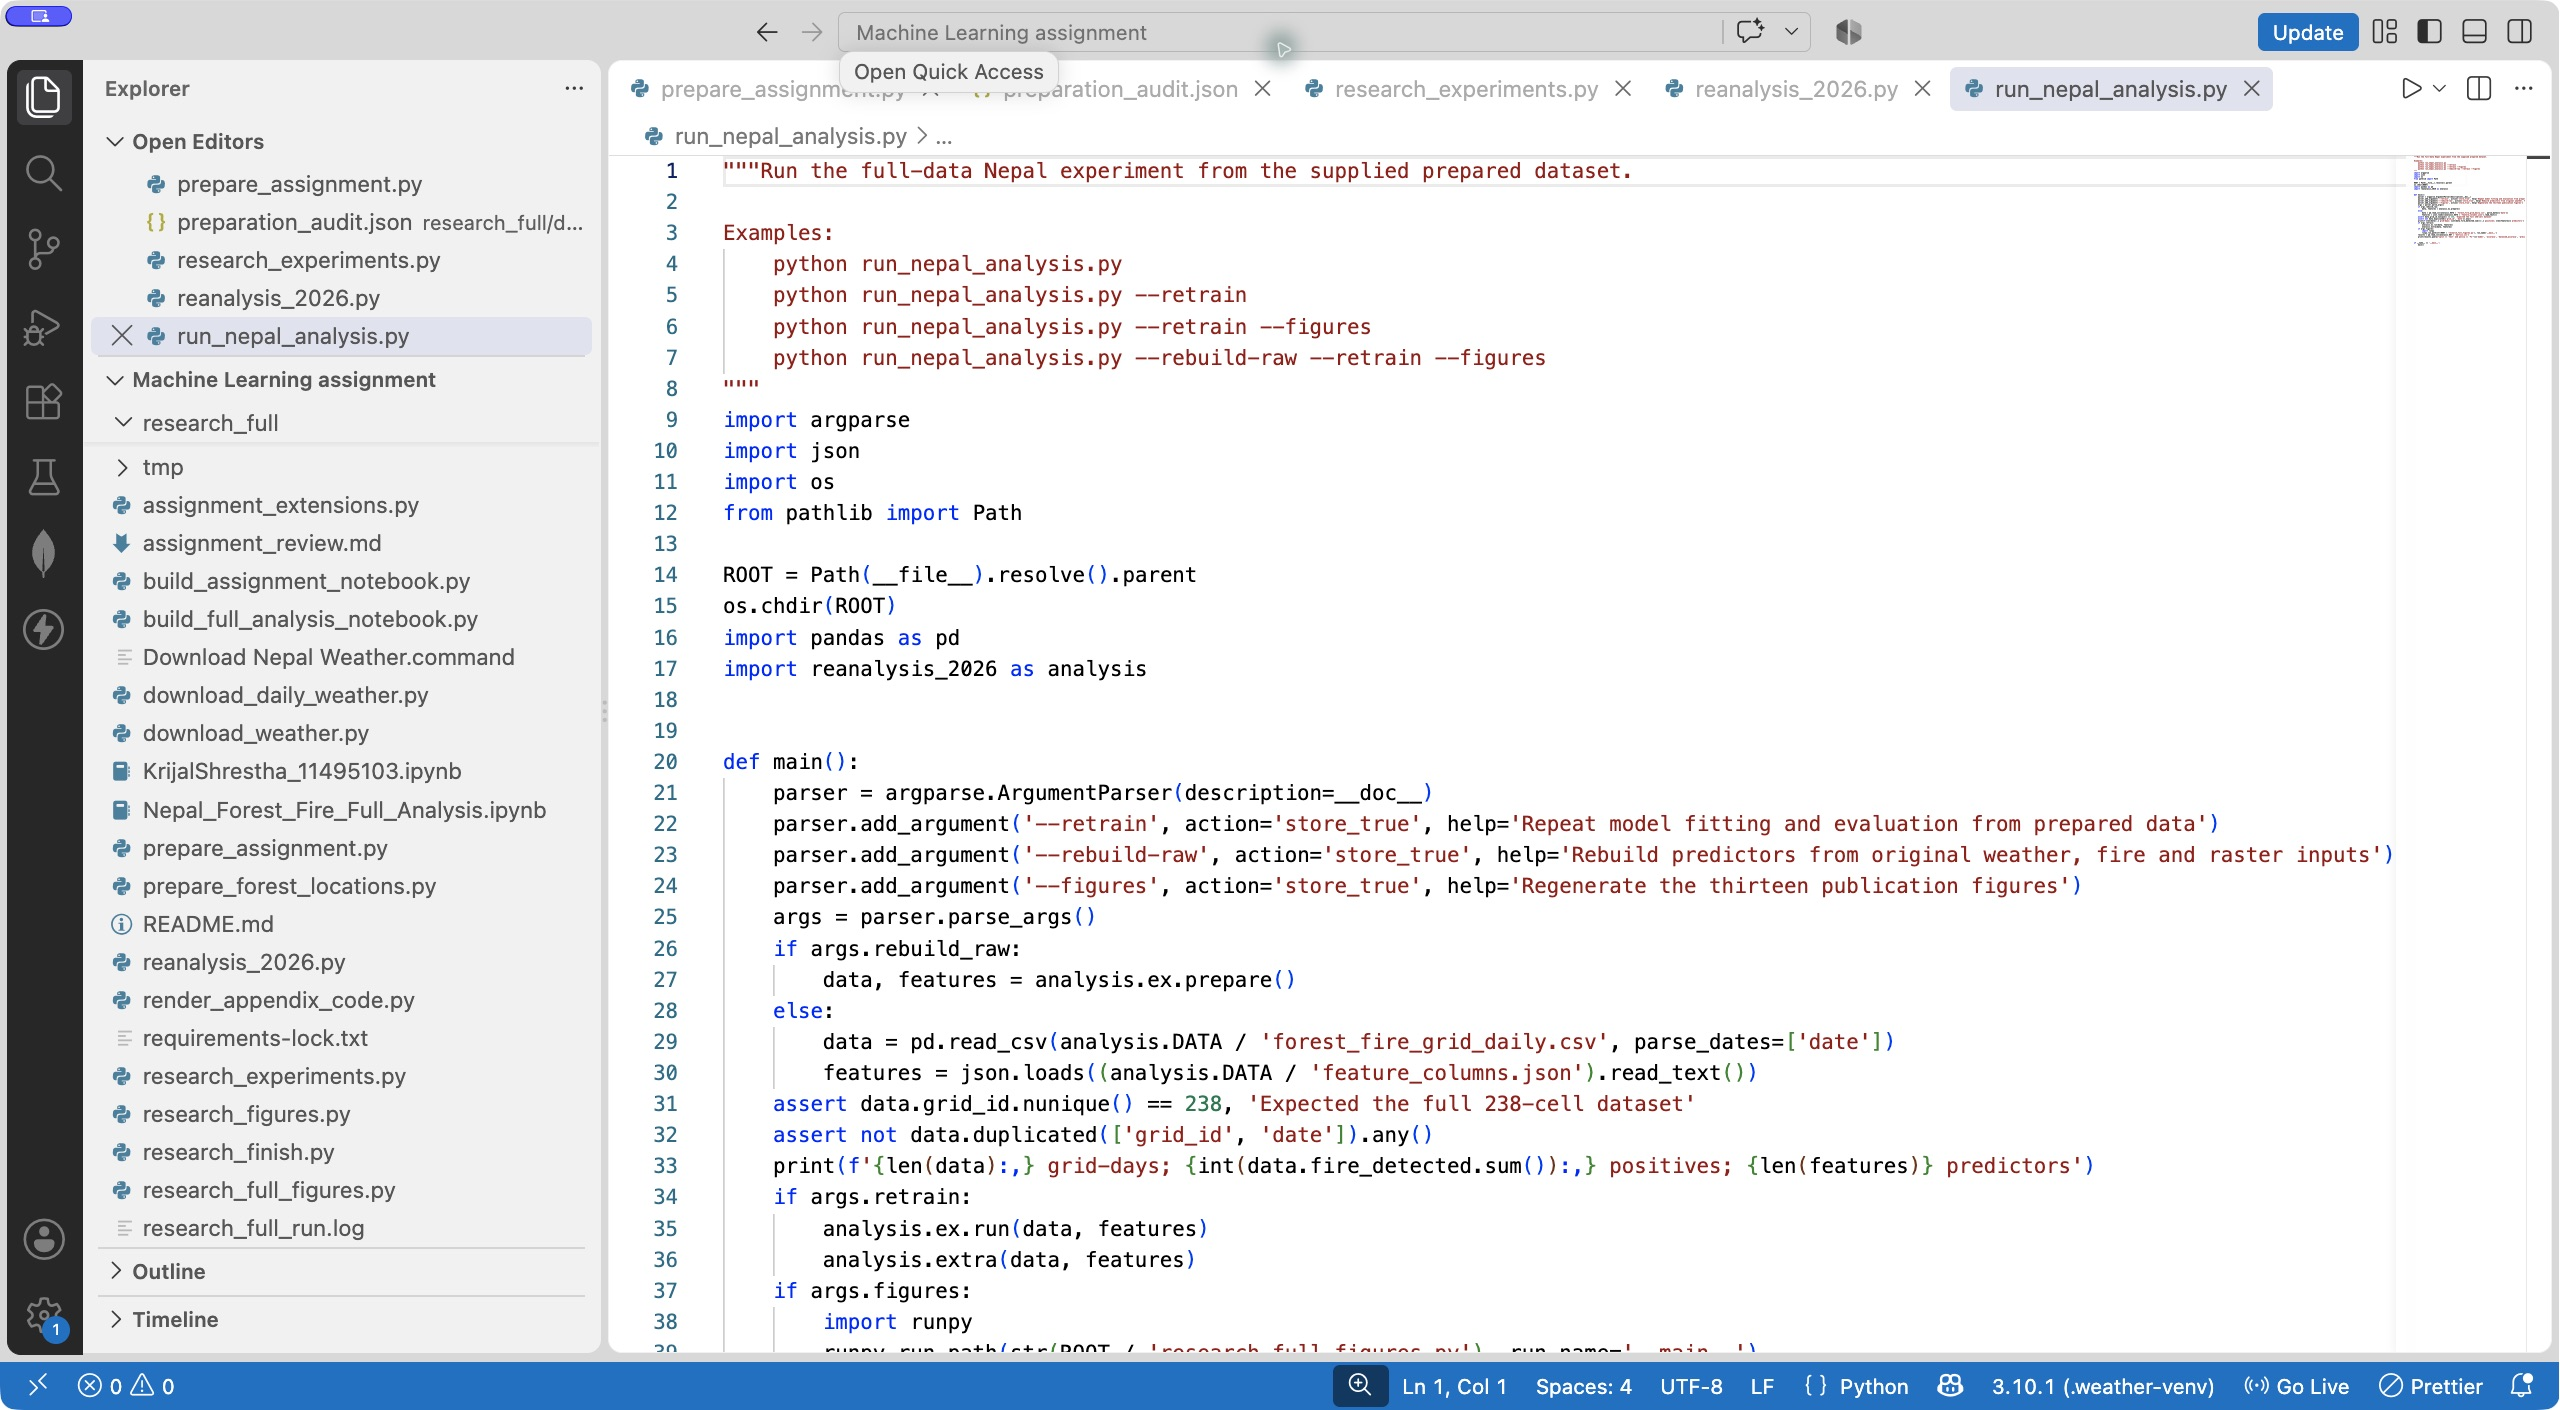
\includegraphics[trim=0 0 0 100,clip,width=\columnwidth]{images/vscode_10_runner.png}
\caption{Visual Studio Code: The runnable analysis entry point and its command-line options.}
\label{fig:appendix-vscode-9}
\end{figure}

\begin{figure}[!htbp]
\centering
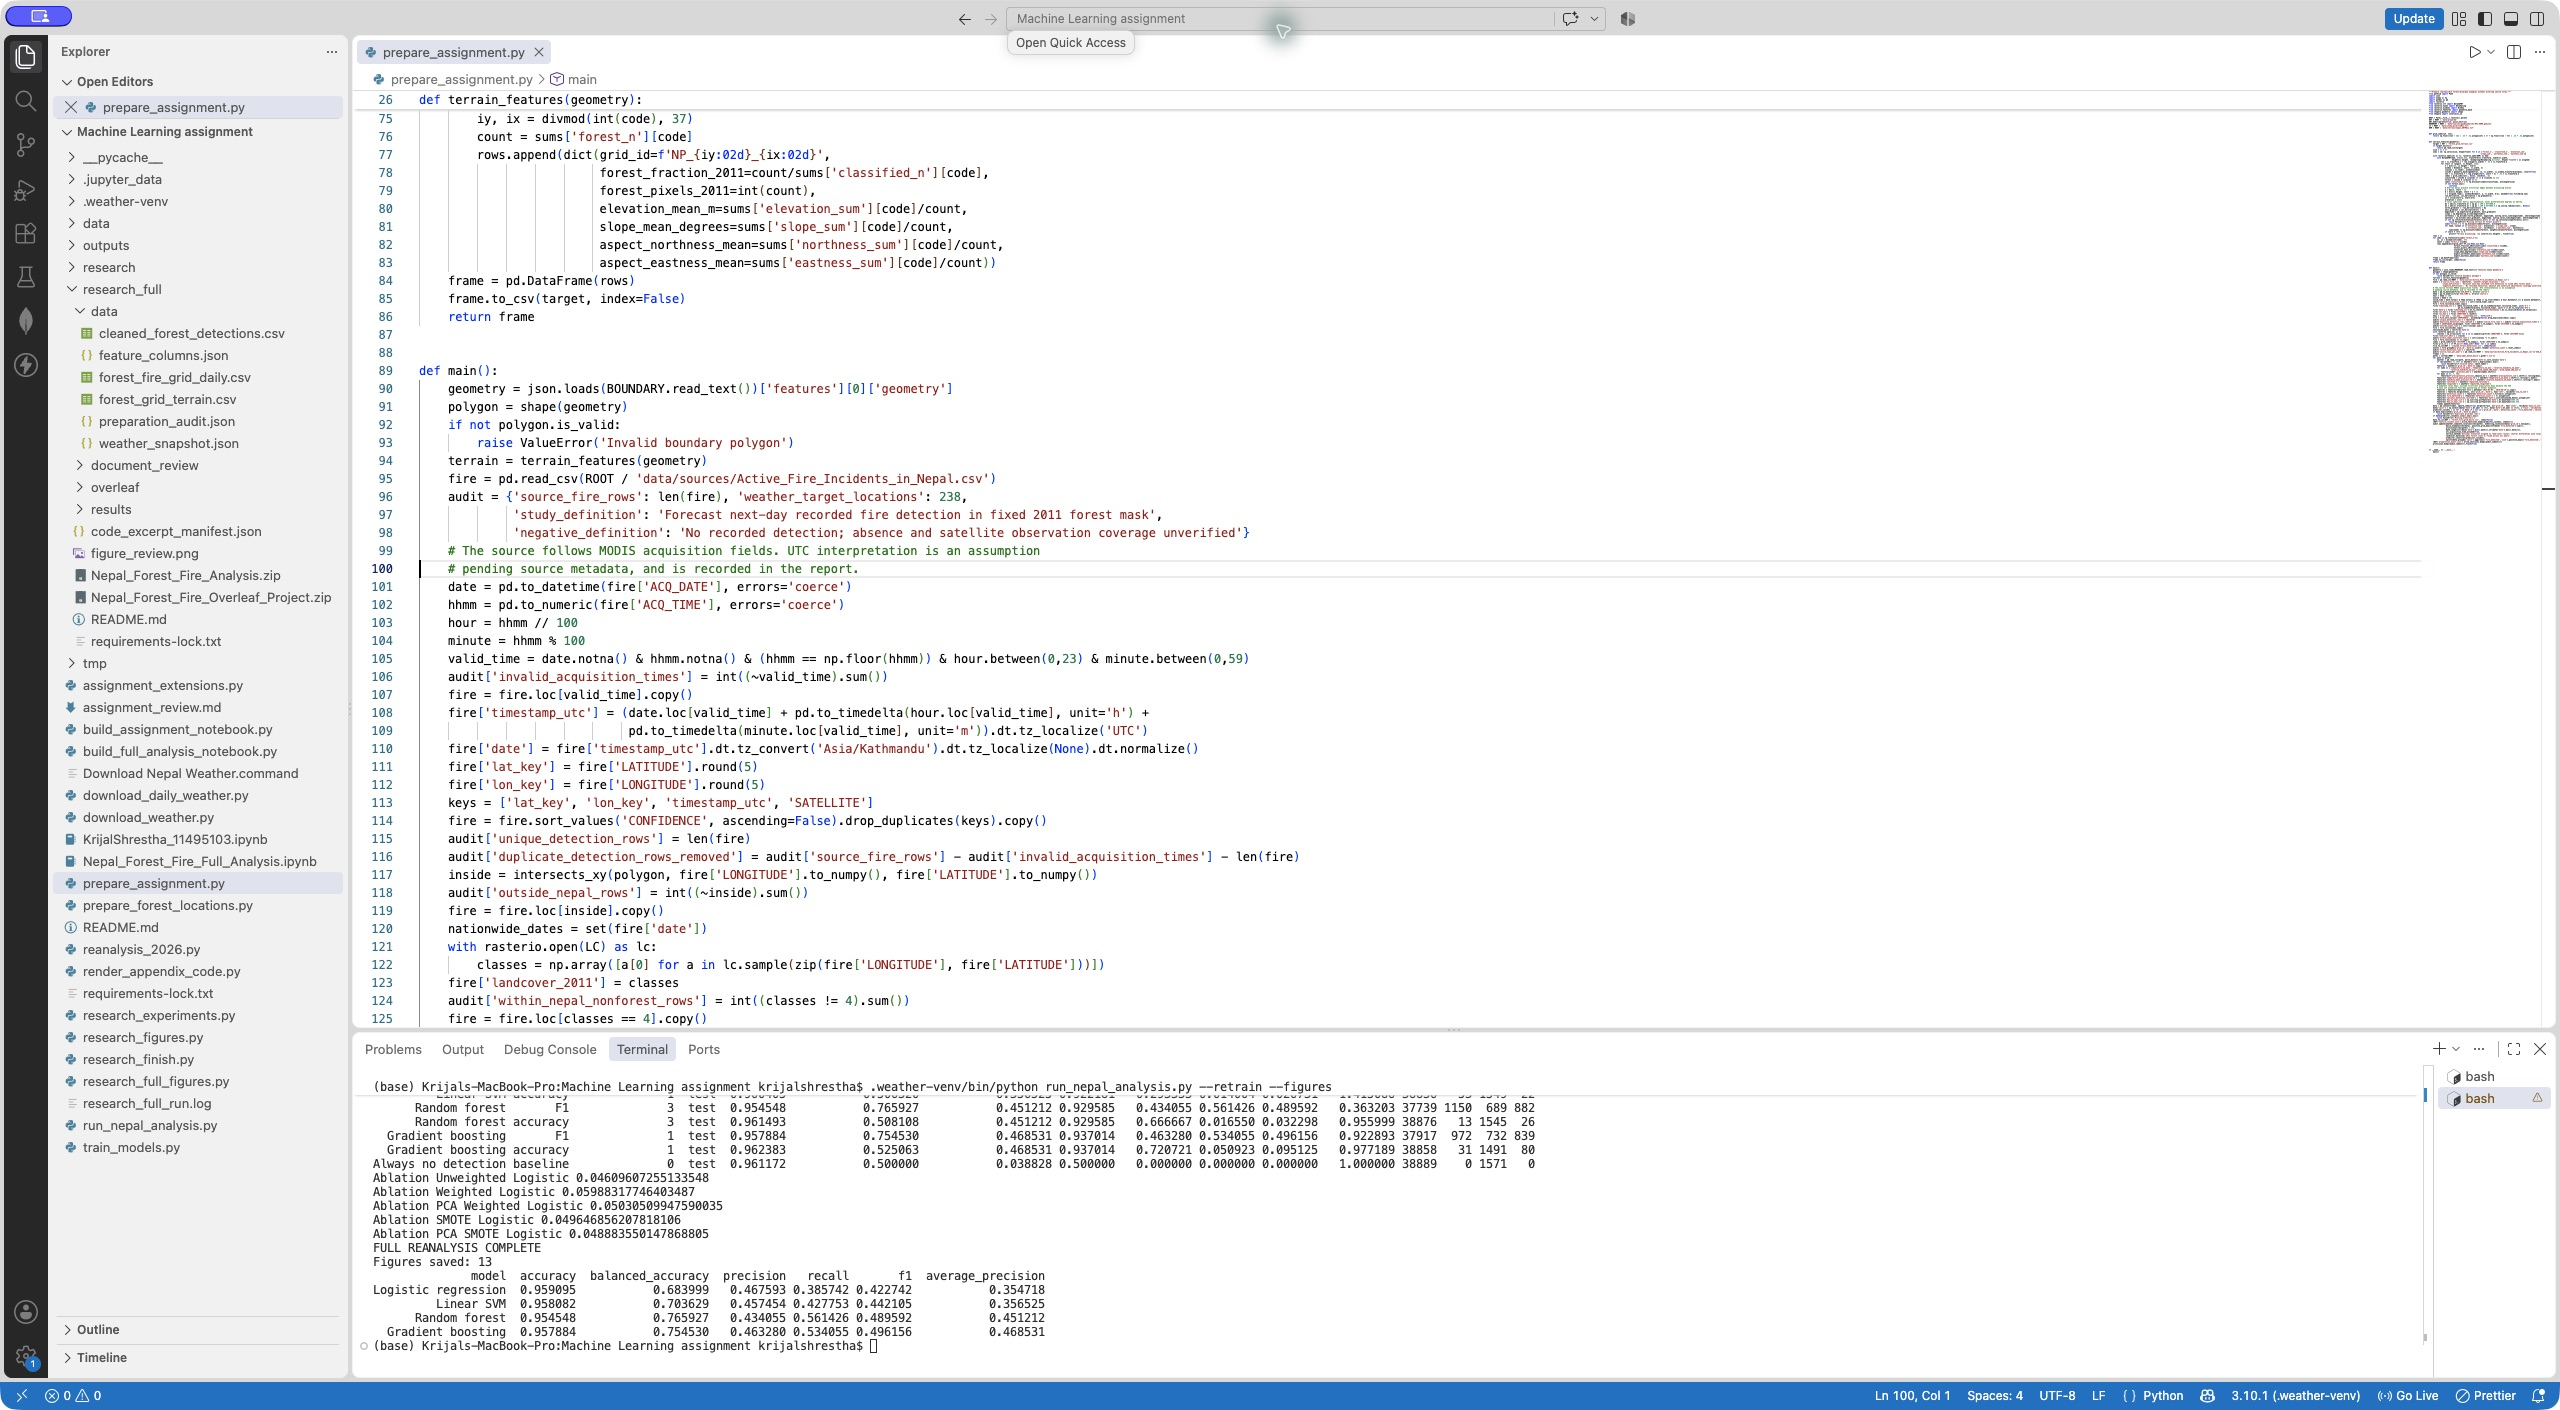
\includegraphics[trim=0 0 0 100,clip,width=\columnwidth]{images/vscode_01_code_and_run.png}
\caption{Visual Studio Code: Project source alongside the completed analysis output in the VS Code terminal.}
\label{fig:appendix-vscode-10}
\end{figure}

\begin{figure}[!htbp]
\centering
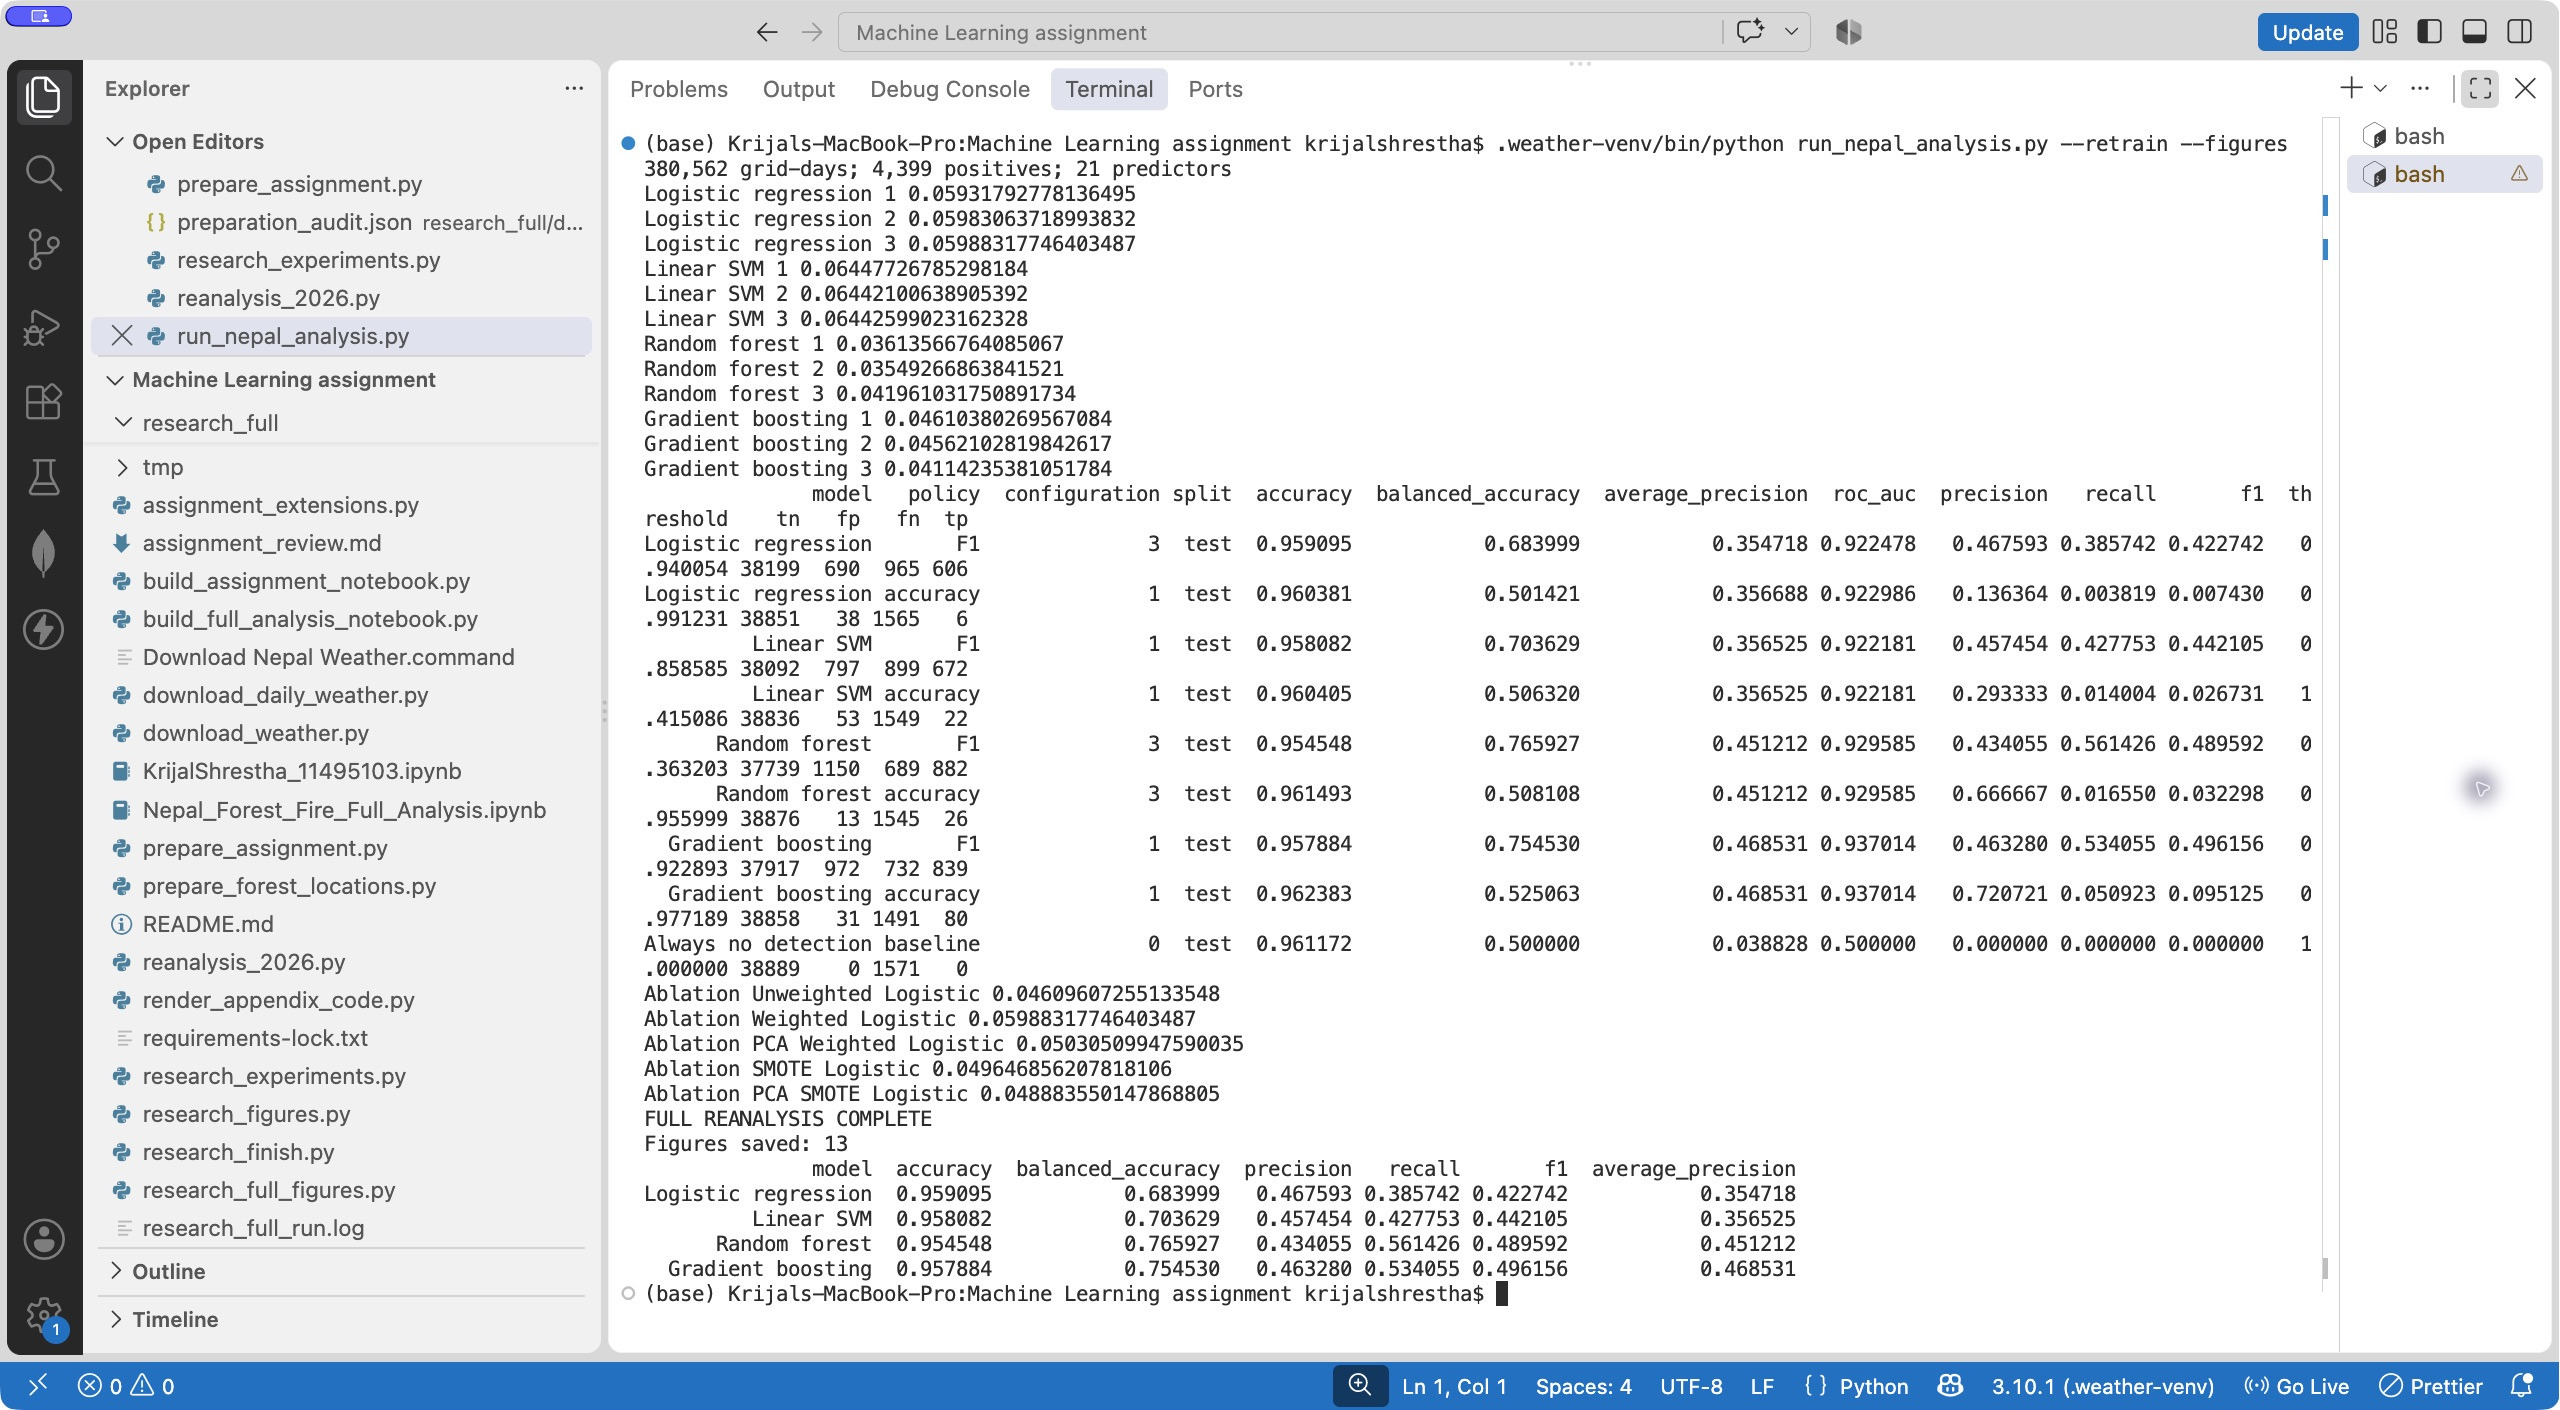
\includegraphics[trim=0 0 0 100,clip,width=\columnwidth]{images/vscode_11_completed_run.png}
\caption{Visual Studio Code: The completed training and figure-generation command, measured outputs and completion message.}
\label{fig:appendix-vscode-11}
\end{figure}

\end{document}
